% Build: cd docs/reports/reconstruction && latexmk -xelatex rk_reconstruction_status_20260416_zh.tex
\documentclass[a4paper, 11pt]{article}

\usepackage[margin=2.4cm]{geometry}
\usepackage{ctex}            % 中文支持
\usepackage{amsmath,amssymb}
\usepackage{booktabs}
\usepackage{multirow}
\usepackage{siunitx}
\usepackage{xcolor}
\usepackage{hyperref}
\usepackage{enumitem}
\usepackage{float}
\usepackage{graphicx}
\usepackage{tikz}
\usetikzlibrary{arrows.meta,positioning,calc}
\usepackage{algorithm}
\usepackage{algpseudocode}

\definecolor{goodgreen}{RGB}{34,139,34}
\definecolor{warnred}{RGB}{200,50,50}

\hypersetup{
  colorlinks=true,
  linkcolor=blue!60!black,
  citecolor=blue!60!black,
  urlcolor=blue!60!black,
}

\title{\textbf{PDC 靶点动量重建算法与误差分析\\——当前状态详细报告}}
\author{TBT \\ RIKEN 仁科中心 / DPOL 实验}
\date{2026 年 4 月 16 日}

\begin{document}
\maketitle
\tableofcontents
\newpage

% ============================================================
\section{引言}
% ============================================================

DPOL（Deuteron Polarization）实验在 RIKEN SAMURAI 终端进行，旨在精确测量氘核极化观测量。在实验数据处理链中，将 PDC（Proportional Drift Chamber，比例漂移室）上的探测器命中坐标反推出靶点处的粒子动量矢量是至关重要的环节。

本报告详细描述了当前 PDC $\to$ 靶点动量重建管线的完整算法框架，包括：
\begin{enumerate}[nosep]
  \item 基于 Runge-Kutta 四阶积分的相对论轨迹模型；
  \item 丝坐标系中的残差构建与二维白化；
  \item Levenberg-Marquardt 最小二乘优化与多起点初始化策略；
  \item 五种互补的误差分析方法（Fisher 信息、蒙特卡洛非线性传播、Profile Likelihood、Laplace 后验、MCMC）；
  \item 由谱仪几何推导的 Cramér-Rao 理论分辨极限；
  \item 当前 E2E（端到端）测试结果及与神经网络后端的对比。
\end{enumerate}

% ============================================================
\section{实验装置与坐标系统}
% ============================================================

\subsection{两个坐标系：lab 系与靶（beam-as-Z）系}
\label{sec:frame_convention}

本报告涉及两个右手直角坐标系，区分它们对理解 $p_x$ 系统偏差至关重要：

\begin{itemize}
  \item \textbf{Lab 系（Geant4 世界坐标系）}：
    $+z$ 沿 SAMURAI 实验厅的标称束流方向，$+y$ 竖直向上，$+x$ 水平向外。
    所有 PDC 命中、磁场表、Runge--Kutta 轨迹积分、以及最小二乘拟合的内部运算都在此坐标系下完成。
  \item \textbf{靶系（beam-as-Z 系，事件发生器输入帧）}：
    以“入射束流方向为 $+z$”为约定；相对于 lab 系绕 $y$ 轴旋转 $\alpha_\mathrm{tgt} = 3^\circ$
    （靶倾角，同节所述）。Geant4 正向模拟对初级动量执行 $R_y(-\alpha_\mathrm{tgt})$
    生成实验室帧方向（\texttt{DeutPrimaryGeneratorAction.cc}），但 ROOT 输出中的
    \texttt{truth\_proton\_p4} 仍保留为输入的 beam-as-Z 系分量（\texttt{fMomentum} 未被回写）。
\end{itemize}

\textbf{本报告所有 truth vs.\ reco 的比较、所有直方图均在靶系下给出。}
在重建输出端（\texttt{apps/run\_reconstruction/main.cc} 和 \texttt{apps/tools/analyze\_pdc\_rk\_error.cc}），
重建结果在写出前统一施加 $R_y(+\alpha_\mathrm{tgt})$ 把 lab 系量旋回靶系；
动量 $3\times 3$ 协方差按 $\Sigma' = R\,\Sigma\,R^\mathrm{T}$ 同步旋转，
$px/py/pz$ 的 Fisher/Laplace 区间用旋转后的对角高斯重建；MCMC/Profile 的非对称分位信息退化为高斯回退
（原采样未保留于 \texttt{RecoResult} 中）。$|\vec p\,|$ 在绕 $y$ 的旋转下不变，
故 \texttt{reco\_proton\_p\_sigma}、\texttt{p\_lower68} 等 $|\vec p|$ 相关字段保持不变。

\textbf{2026-04-19 修复前}，重建端未施加此旋转，造成系统性伪 $p_x$ 偏差
$\Delta p_x \approx p_x(\cos\alpha - 1) - p_z\sin\alpha$；对 $\alpha = 3^\circ$、
$p_z \approx 627\;\mathrm{MeV}/c$ 的质子，$\Delta p_x \approx -33\;\mathrm{MeV}/c$
（若 $p_z \approx 1\;\mathrm{GeV}/c$，则 $\Delta p_x \approx -52\;\mathrm{MeV}/c$）。
修复后 $p_x$ Fisher 68\% 覆盖率从 $\approx 0.05$ 恢复到 $\approx 0.80$。
2026-04-17 及更早日期生成的 PNG 图受此偏差影响；本报告中所有图均为 2026-04-19 修复后重新生成。
共享旋转工具位于 \texttt{libs/analysis\_pdc\_reco/include/PDCFrameRotation.hh}。

\subsection{SAMURAI 磁谱仪几何}

实验坐标系定义：束流方向为 $+z$，竖直方向为 $y$，水平方向为 $x$。主要几何元素：

\begin{table}[H]
\centering
\caption{关键几何参数}
\begin{tabular}{lrl}
\toprule
参数 & 数值 & 说明 \\
\midrule
靶点位置 & $z \approx -1070\;\mathrm{mm}$ & 磁铁内部，旋转 $3^\circ$ \\
SAMURAI 偶极磁铁 & $B \approx 1.15\;\mathrm{T}$ & 中心在原点，绕 $y$ 轴旋转 $30^\circ$ \\
磁铁尺寸（半长） & $3350 \times 2320 \times 1750\;\mathrm{mm}$ & $x \times y \times z$，靶在其中 \\
PDC1 位置 & $z \approx 4000\;\mathrm{mm}$ & 第一平面漂移室 \\
PDC2 位置 & $z \approx 5000\;\mathrm{mm}$ & 第二平面漂移室 \\
PDC 倾斜角 & $\theta_\mathrm{PDC} = 57^\circ$ & 探测器相对束流轴的旋转角 \\
PDC 位置分辨 & $\sigma_{uv} = 0.5\;\mathrm{mm}$ & Geant4 模拟中的 smearing 参数 \\
\bottomrule
\end{tabular}
\end{table}

典型的重建目标粒子为质子，动量约 $|\vec{p}| \approx 635\;\mathrm{MeV}/c$，其中 $p_z \approx 627\;\mathrm{MeV}/c$。

\begin{figure}[H]
\centering
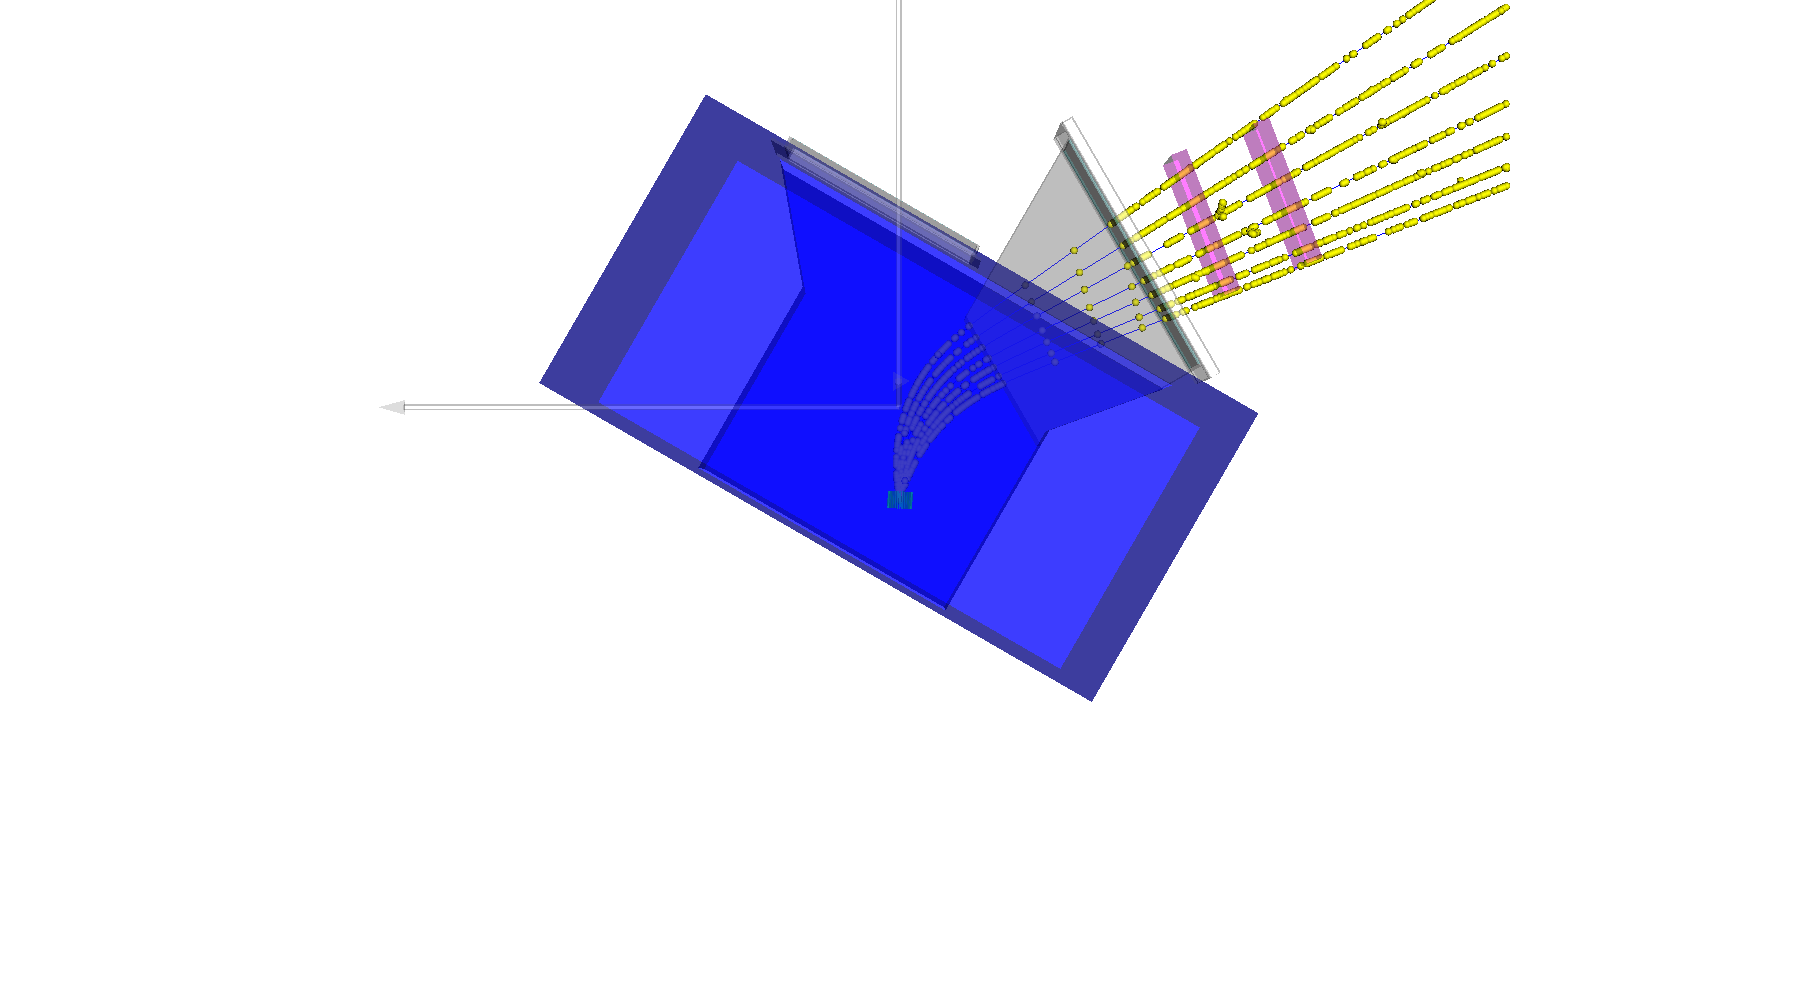
\includegraphics[width=0.92\textwidth]{figures/geometry/samurai_geometry_xz.png}
\caption{SAMURAI 磁谱仪 $xz$ 平面俯视图（从 Geant4 VRML 导出渲染）。蓝色：SAMURAI 偶极磁铁（绕 $y$ 轴旋转 $30^\circ$，中心在原点）；绿色（磁铁内部）：靶点（$z \approx -1070\;\mathrm{mm}$）；黄色：质子轨迹在磁场中弯曲（$p_z = 627\;\mathrm{MeV}/c$，$p_x$ 扫描）；粉色：PDC1（$z \approx 4000\;\mathrm{mm}$）和 PDC2（$z \approx 5000\;\mathrm{mm}$）漂移室。}
\end{figure}

\subsection{PDC 丝坐标系}
\label{sec:wire_coord}

PDC 探测器在每个平面提供两个一维坐标量 $u$ 和 $v$，分别对应沿两组丝方向的投影位置。在 Geant4 模拟中（\texttt{PDCSimAna}），丝坐标的定义如下：

首先将命中点的实验室坐标相对于 PDC 中心做差，然后绕 $y$ 轴旋转 PDC 倾斜角 $\theta$，得到旋转后的局部坐标：
\begin{equation}
  x_\mathrm{rot} = \Delta x \cos\theta - \Delta z \sin\theta,
\end{equation}
其中 $\Delta x = x - x_\mathrm{PDC}$，$\Delta z = z - z_\mathrm{PDC}$。

丝坐标定义为：
\begin{equation}
  u = \frac{x_\mathrm{rot} + y}{\sqrt{2}}, \qquad
  v = \frac{-x_\mathrm{rot} + y}{\sqrt{2}}.
  \label{eq:wire_coord}
\end{equation}

对上式求微分可得丝方向在实验室坐标系中的单位矢量：
\begin{equation}
  \hat{u} = \frac{1}{\sqrt{2}}
  \begin{pmatrix} \cos\theta \\ +1 \\ \sin\theta \end{pmatrix}, \qquad
  \hat{v} = \frac{1}{\sqrt{2}}
  \begin{pmatrix} \cos\theta \\ -1 \\ \sin\theta \end{pmatrix}.
  \label{eq:wire_dir}
\end{equation}

\paragraph{关键物理意义。}
$\hat{u}$ 和 $\hat{v}$ 都具有非零的 $z$ 分量 $\sin\theta/\sqrt{2} \approx 0.593$（当 $\theta = 57^\circ$ 时）。SAMURAI 磁场在 $xz$ 平面弯曲粒子轨迹，轨迹的曲率信息主要编码在 $z$ 方向的位移中。因此，丝方向的 $z$ 分量直接携带了动量信息。若错误地使用纯 $xy$ 平面投影（即令 $\hat{u}$、$\hat{v}$ 的 $z$ 分量为零），则残差中将完全丢失曲率信号，导致 fitter 无法确定动量。

由式~\eqref{eq:wire_coord} 可反解出实验室坐标：
\begin{equation}
  y = \frac{u + v}{\sqrt{2}}, \qquad
  x_\mathrm{rot} = \frac{u - v}{\sqrt{2}}.
\end{equation}

再经过逆旋转恢复实验室坐标 $(x, y, z)$：
\begin{equation}
  x = x_\mathrm{rot} \cos\theta + x_\mathrm{PDC}, \qquad
  z = x_\mathrm{rot} \sin\theta + z_\mathrm{PDC}.
\end{equation}

% ============================================================
\section{相对论轨迹模型}
% ============================================================

\subsection{运动方程}

质量为 $m$、电荷为 $q$ 的带电粒子在外磁场 $\vec{B}(\vec{r})$ 中的相对论运动方程为：
\begin{align}
  \frac{d\vec{r}}{dt} &= \vec{v} = \frac{\vec{p}\,c^2}{E}, \label{eq:eom_r} \\
  \frac{d\vec{p}}{dt} &= q\,\vec{v} \times \vec{B}(\vec{r}), \label{eq:eom_p}
\end{align}
其中能量 $E = \sqrt{|\vec{p}|^2 c^2 + m^2 c^4}$。在我们的单位系统（位置 mm，时间 ns，动量 MeV/$c$，磁场 T）中，转换常数为：
\begin{equation}
  q_e \cdot c = 89.876\;\frac{\mathrm{MeV}}{\mathrm{c \cdot T \cdot ns}}.
\end{equation}

洛伦兹力与速度正交，因此 $|\vec{p}|$ 在磁场中守恒（当前模型不含 $dE/dx$ 能量损失）。在旋转了 $30^\circ$ 的 SAMURAI 磁场（以 $B_y$ 分量为主导）中，粒子的主要偏转发生在 $xz$ 平面内。

\subsection{四阶 Runge-Kutta 积分}

将位置和动量合并为状态矢量 $\vec{Y} = (\vec{r}, \vec{p})$，运动方程写成 $d\vec{Y}/dt = f(\vec{Y})$ 的形式。RK4 方法以固定时间步长 $\Delta t$ 对其数值积分：
\begin{align}
  \vec{K}_1 &= f\bigl(\vec{Y}_n\bigr), \\
  \vec{K}_2 &= f\bigl(\vec{Y}_n + \tfrac{\Delta t}{2}\vec{K}_1\bigr), \\
  \vec{K}_3 &= f\bigl(\vec{Y}_n + \tfrac{\Delta t}{2}\vec{K}_2\bigr), \\
  \vec{K}_4 &= f\bigl(\vec{Y}_n + \Delta t\,\vec{K}_3\bigr), \\
  \vec{Y}_{n+1} &= \vec{Y}_n + \frac{\Delta t}{6}
  \bigl(\vec{K}_1 + 2\vec{K}_2 + 2\vec{K}_3 + \vec{K}_4\bigr).
  \label{eq:rk4}
\end{align}

每个时间步需要查询磁场图 $\vec{B}(\vec{r})$ 四次。轨迹以离散点列 $\{(\vec{r}_i, \vec{p}_i, t_i)\}$ 的形式存储。

\paragraph{实现参数。}
默认步长 $\Delta t \sim 0.1\;\mathrm{ns}$，对应约 $30\;\mathrm{mm}$ 的空间步长。从靶点到 PDC2 共约 150--200 步。轨迹的最大传播距离设为 $\max(1500, d_\mathrm{far} + 1500)\;\mathrm{mm}$，其中 $d_\mathrm{far}$ 为起点到较远 PDC 的距离，确保在强曲率下轨迹仍能到达两个 PDC 平面。

% ============================================================
\section{最小二乘拟合}
% ============================================================

\subsection{参数化}

重建的待定参数用五维状态矢量描述：
\begin{equation}
  \vec{\alpha} = (\delta x,\; \delta y,\; u,\; v,\; p),
\end{equation}
各参数的物理意义：
\begin{itemize}[nosep]
  \item $\delta x$，$\delta y$：靶点位置相对于标称位置的偏移量（mm）；
  \item $u = p_x / p_z$，$v = p_y / p_z$：出射方向的正切值（无量纲）；
  \item $p = |\vec{p}|$：动量模（MeV/$c$）。
\end{itemize}

直接以 $p$ 而非 $q = \mathrm{charge}/p$ 作为参数，使先验分布和参数截断都直接作用在物理量上，物理意义更为清晰。

由 $(u, v, p)$ 重建动量分量：
\begin{equation}
  p_z = \frac{p}{\sqrt{1 + u^2 + v^2}}, \qquad
  p_x = u \cdot p_z, \qquad
  p_y = v \cdot p_z.
  \label{eq:momentum_from_uvp}
\end{equation}

\subsection{拟合模式}

系统支持三种拟合模式，区别在于自由参数的数目和约束条件：

\begin{table}[H]
\centering
\caption{三种拟合模式的参数与残差配置}
\label{tab:fit_modes}
\begin{tabular}{lccccc}
\toprule
模式 & 自由参数 & PDC 残差 & 靶约束残差 & $N_\mathrm{res}$ & $N_\mathrm{dof}$ \\
\midrule
\texttt{kFixedTargetPdcOnly} & $u, v, p$ & 4 & 0 & 4 & 1 \\
\texttt{kTwoPointBackprop} & $u, v, p$ & 4 & 0 & 4 & 1 \\
\texttt{kThreePointFree} & $\delta x, \delta y, u, v, p$ & 4 & 2 & 6 & 1 \\
\bottomrule
\end{tabular}
\end{table}

\texttt{kFixedTargetPdcOnly} 和 \texttt{kTwoPointBackprop} 使用相同的参数布局（固定靶点），仅在历史上有不同的初始化逻辑（现已统一）。\texttt{kThreePointFree} 额外释放靶点位置 $(\delta x, \delta y)$，并引入软先验 $w_5 = \delta x / \sigma_\mathrm{tgt}$，$w_6 = \delta y / \sigma_\mathrm{tgt}$ 作为正则化。

\subsection{残差构建}
\label{sec:residual}

对于给定的参数状态 $\vec{\alpha}$，重建过程如下：

\paragraph{步骤一：轨迹传播。}
以靶点位置（加偏移 $\delta x$, $\delta y$）为起点，以式~\eqref{eq:momentum_from_uvp} 构造初始动量矢量，调用 RK4 积分器沿磁场传播轨迹直到超过 PDC2。

\paragraph{步骤二：最近点匹配。}
在轨迹点列中搜索距 PDC1 命中点 $\vec{r}_1^\mathrm{meas}$ 和 PDC2 命中点 $\vec{r}_2^\mathrm{meas}$ 最近的轨迹点，分别记为 $\vec{r}_1^\mathrm{traj}$ 和 $\vec{r}_2^\mathrm{traj}$。

\paragraph{步骤三：丝坐标投影。}
计算三维位移并投影到丝方向：
\begin{align}
  r_u^{(k)} &= \bigl(\vec{r}_k^\mathrm{traj} - \vec{r}_k^\mathrm{meas}\bigr) \cdot \hat{u}, \label{eq:res_u} \\
  r_v^{(k)} &= \bigl(\vec{r}_k^\mathrm{traj} - \vec{r}_k^\mathrm{meas}\bigr) \cdot \hat{v}, \label{eq:res_v}
\end{align}
其中 $k = 1, 2$ 对应 PDC1 和 PDC2。离面分量（即与 $\hat{u}$、$\hat{v}$ 都正交的方向）被丢弃——它不是 PDC 的测量量。

\paragraph{步骤四：二维 Cholesky 白化。}
每个平面的测量误差由二维协方差矩阵 $C$ 描述：
\begin{equation}
  C = \begin{pmatrix}
    \sigma_u^2 & \rho\,\sigma_u\,\sigma_v \\
    \rho\,\sigma_u\,\sigma_v & \sigma_v^2
  \end{pmatrix},
  \label{eq:cov_matrix}
\end{equation}
其中 $\sigma_u$、$\sigma_v$ 分别为 $u$、$v$ 方向的位置分辨，$\rho$ 为 $u$-$v$ 关联系数。对 $C$ 做 Cholesky 分解 $C = LL^T$，白化变换为：
\begin{equation}
  \begin{pmatrix} w_1 \\ w_2 \end{pmatrix}
  = L^{-1}
  \begin{pmatrix} r_u \\ r_v \end{pmatrix}.
  \label{eq:whitening}
\end{equation}

白化后的残差 $w_1$、$w_2$ 是独立的标准正态变量（均值为零、方差为一），可以直接进入 $\chi^2$ 求和。

\subsection{$\chi^2$ 目标函数}

总的加权残差平方和为：
\begin{equation}
  \chi^2(\vec{\alpha}) = \sum_{i=1}^{N_\mathrm{res}} w_i^2(\vec{\alpha}),
  \label{eq:chi2}
\end{equation}
其中 $N_\mathrm{res} = 4$（固定靶点模式）或 $6$（自由靶点模式），$N_\mathrm{dof} = N_\mathrm{res} - N_\mathrm{param} = 1$。

% ============================================================
\subsection{Levenberg-Marquardt 优化}
\label{sec:lm}

\subsubsection{数值 Jacobian}

残差 Jacobian 矩阵 $J_{ij} = \partial w_i / \partial \alpha_j$ 通过中心差分法计算。对每个活跃参数 $\alpha_j$，分别在 $\alpha_j \pm h_j$ 处评估残差矢量，取差商：
\begin{equation}
  J_{ij} \approx \frac{w_i(\vec{\alpha} + h_j \vec{e}_j) - w_i(\vec{\alpha} - h_j \vec{e}_j)}{2h_j},
\end{equation}
其中步长 $h_j$ 根据参数类型自适应选取：
\begin{itemize}[nosep]
  \item $\delta x$, $\delta y$：$h = \max(0.1,\; 0.05\,\sigma_\mathrm{tgt})\;\mathrm{mm}$；
  \item $u$, $v$：$h = \max(10^{-4},\; 0.01 \cdot \max(|u|, 0.05))$；
  \item $p$：$h = \max(0.5,\; 0.001 \cdot p)\;\mathrm{MeV}/c$。
\end{itemize}

每列需要两次完整的 RK 轨迹评估，因此一次 Jacobian 计算需要 $2 N_\mathrm{param}$ 次轨迹传播（6 次或 10 次）。

\subsubsection{LM 迭代}

在第 $n$ 次迭代中，法方程为：
\begin{equation}
  \bigl(J^T J + \lambda \cdot \mathrm{diag}(J^T J)\bigr)\,\Delta\vec{\alpha}
  = -J^T \vec{w},
  \label{eq:lm_normal}
\end{equation}
其中 $\lambda$ 是阻尼参数。当 $\lambda$ 很大时趋于梯度下降（步长短、方向稳定），$\lambda$ 很小时趋于 Gauss-Newton（二次收敛）。

法方程通过 SVD 分解求解，避免了 $(J^TJ)$ 接近奇异时的数值不稳定。更新规则：
\begin{itemize}[nosep]
  \item 若 $\chi^2_\mathrm{new} < \chi^2_\mathrm{old}$（接受）：$\lambda \to \lambda / 3$；
  \item 否则（拒绝）：$\lambda \to 4\lambda$。
\end{itemize}

收敛条件（满足任一即停止）：
\begin{itemize}[nosep]
  \item $\chi^2$ 改善量 $< 10^{-8}$；
  \item 参数步长 $\|\Delta\vec{\alpha}\| < 10^{-5}$；
  \item $\lambda$ 达到上限（收敛失败）。
\end{itemize}

\subsection{初始化：粗网格搜索与多起点策略}
\label{sec:grid_search}

\subsubsection{初始化困难}

从靶点到 PDC 的直线方向无法作为良好的初始猜测。对于 $635\;\mathrm{MeV}/c$ 的质子在 $1.15\;\mathrm{T}$ 磁场中，偏转角约 $25^\circ$。直线方向与真实出射方向的偏差巨大，导致 LM 优化从极大的残差出发，极易陷入局部最小值。

\subsubsection{粗网格搜索}

在参数空间 $(u, v, p)$ 上构建 $7 \times 3 \times 5 = 105$ 个候选点的粗网格：
\begin{itemize}[nosep]
  \item $u$ 方向：以直线估计值 $u_\mathrm{line}$ 为中心，范围 $[u_\mathrm{line} - 1.0,\; u_\mathrm{line} + 1.0]$，7 个等距点。此范围覆盖 $\pm 45^\circ$ 的方向偏差，足以包含磁场导致的偏转。
  \item $v$ 方向：以直线估计值 $v_\mathrm{line}$ 为中心，范围 $[v_\mathrm{line} - 0.3,\; v_\mathrm{line} + 0.3]$，3 个等距点。$v$ 方向偏转较小（磁场弯曲主要在 $xz$ 平面）。
  \item $p$ 方向：5 个固定值 $\{200, 400, 700, 1200, 2000\}\;\mathrm{MeV}/c$，覆盖广泛的动量范围。
\end{itemize}

对每个候选点调用 \texttt{Evaluate()} 评估 $\chi^2$（一次完整 RK 轨迹传播），将结果按 $\chi^2$ 从小到大排序。计算成本约 $105 \times 0.1\;\mathrm{ms} \approx 10\;\mathrm{ms}$。

\subsubsection{多起点优化}

选取网格中 $\chi^2$ 最低的 5 个候选作为 LM 的起始状态。对每个起始状态独立运行完整的 LM 优化（不含误差计算），最终选取 $\chi^2$ 全局最小的结果。若需要误差分析，再以最优状态为起点运行一次含误差的 LM（已在最小值处，仅需 0--1 次迭代即收敛）。

总计算成本约 $10\;\mathrm{ms}$（网格）$+ 5 \times 10\;\mathrm{ms}$（LM）$\approx 60\;\mathrm{ms}$，对离线重建完全可接受。

\begin{algorithm}[H]
\caption{多起点 RK 动量重建}
\label{alg:multistart}
\begin{algorithmic}[1]
\State \textbf{输入}：PDC1/PDC2 命中坐标，靶点位置，磁场图
\State 计算直线方向 $(u_\mathrm{line}, v_\mathrm{line})$
\State 生成 $7 \times 3 \times 5 = 105$ 个 $(u, v, p)$ 候选
\For{每个候选 $(u_k, v_k, p_k)$}
  \State 评估 $\chi^2_k \gets \texttt{Evaluate}(u_k, v_k, p_k)$
\EndFor
\State 按 $\chi^2$ 排序，选取前 5 个候选
\For{每个候选 $i \in \{1, \dots, 5\}$}
  \State 从候选 $i$ 出发运行 LM $\to$ 结果 $(\vec{\alpha}_i^{*}, {\chi^2_i}^{*})$
\EndFor
\State $\vec{\alpha}^{*} \gets \arg\min_i {\chi^2_i}^{*}$
\If{需要误差分析}
  \State 从 $\vec{\alpha}^*$ 出发运行 LM（含 Fisher 协方差计算）
\EndIf
\State \textbf{输出}：最优参数 $\vec{\alpha}^{*}$，$\chi^2$，协方差矩阵
\end{algorithmic}
\end{algorithm}

% ============================================================
\section{误差分析}
\label{sec:error}
% ============================================================

本节详细推导六种误差分析方法，并明确说明每个数学量在本重建问题中对应的物理量。

\subsection{问题设定与符号约定}

为方便读者理解后续推导，首先定义本重建问题的核心数学结构。

\paragraph{参数空间。}
以 \texttt{kFixedTargetPdcOnly} 模式为例（其他模式类似），待拟合的参数为三维矢量：
\begin{equation}
  \vec{\alpha} = (u,\; v,\; p),
  \label{eq:param_vec}
\end{equation}
其中 $u = p_x/p_z$ 和 $v = p_y/p_z$ 是出射方向的正切值（无量纲），$p = |\vec{p}|$ 是动量模（MeV/$c$）。靶点位置 $(\delta x, \delta y)$ 在此模式下固定为零。

\paragraph{测量空间。}
每个 PDC 平面提供两个丝坐标测量值。两个 PDC 共提供 4 个独立测量量，组成测量矢量：
\begin{equation}
  \vec{m} = \bigl(u_1^\mathrm{meas},\; v_1^\mathrm{meas},\; u_2^\mathrm{meas},\; v_2^\mathrm{meas}\bigr),
  \label{eq:meas_vec}
\end{equation}
其中下标 1、2 分别指 PDC1 和 PDC2，$u_k^\mathrm{meas}$ 和 $v_k^\mathrm{meas}$ 是命中位置在丝方向 $\hat{u}$、$\hat{v}$ 上的投影坐标。

\paragraph{前向模型。}
给定参数 $\vec{\alpha}$，重建过程是一个非线性前向模型 $\vec{f}(\vec{\alpha})$：
\begin{enumerate}[nosep]
  \item 由 $(u, v, p)$ 构造初始动量 $\vec{p}_0$（式~\eqref{eq:momentum_from_uvp}）；
  \item 以靶点为起点，调用 RK4 积分器在磁场中传播轨迹；
  \item 在轨迹上找到距 PDC1、PDC2 测量位置最近的点 $\vec{r}_k^\mathrm{traj}(\vec{\alpha})$；
  \item 计算预言的丝坐标：
  \begin{equation}
    f_{2k-1}(\vec{\alpha}) = \vec{r}_k^\mathrm{traj}(\vec{\alpha}) \cdot \hat{u}, \qquad
    f_{2k}(\vec{\alpha}) = \vec{r}_k^\mathrm{traj}(\vec{\alpha}) \cdot \hat{v}, \qquad k=1,2.
  \end{equation}
\end{enumerate}

\paragraph{残差定义。}
原始残差为前向模型预言值与测量值之差（式~\eqref{eq:res_u}、\eqref{eq:res_v}）：
\begin{equation}
  r_i(\vec{\alpha}) = f_i(\vec{\alpha}) - m_i, \qquad i = 1, \dots, 4.
\end{equation}

\paragraph{白化残差。}
经 Cholesky 白化（式~\eqref{eq:whitening}）后，得到标准化残差 $\vec{w}(\vec{\alpha})$：
\begin{equation}
  \vec{w}(\vec{\alpha}) = \bigl(w_1,\; w_2,\; w_3,\; w_4\bigr)^T,
  \label{eq:whitened_residuals}
\end{equation}
其中 $(w_1, w_2)$ 是 PDC1 的白化残差，$(w_3, w_4)$ 是 PDC2 的白化残差。

$\chi^2$ 目标函数即为白化残差的平方和：
\begin{equation}
  \chi^2(\vec{\alpha}) = \sum_{i=1}^{4} w_i^2(\vec{\alpha}), \qquad N_\mathrm{dof} = 4 - 3 = 1.
  \label{eq:chi2_recall}
\end{equation}

\paragraph{自由度。} 4 个独立测量量减去 3 个自由参数，给出 $N_\mathrm{dof} = 1$。这意味着拟合近乎完全约束——仅有 1 个自由度用于检验模型与数据的一致性。

\subsection{方法一：Fisher 信息矩阵}
\label{sec:fisher}

\paragraph{核心思想。}
Fisher 信息矩阵量化了"在最优点附近，$\chi^2$ 对参数变化有多敏感"。$\chi^2$ 对参数越敏感，参数的统计不确定性越小。

\paragraph{Jacobian 矩阵的具体含义。}
残差 Jacobian $J$ 是一个 $4 \times 3$ 矩阵（4 个白化残差对 3 个参数的偏导数）：
\begin{equation}
  J = \frac{\partial \vec{w}}{\partial \vec{\alpha}} =
  \begin{pmatrix}
    \dfrac{\partial w_1}{\partial u} & \dfrac{\partial w_1}{\partial v} & \dfrac{\partial w_1}{\partial p} \\[8pt]
    \dfrac{\partial w_2}{\partial u} & \dfrac{\partial w_2}{\partial v} & \dfrac{\partial w_2}{\partial p} \\[8pt]
    \dfrac{\partial w_3}{\partial u} & \dfrac{\partial w_3}{\partial v} & \dfrac{\partial w_3}{\partial p} \\[8pt]
    \dfrac{\partial w_4}{\partial u} & \dfrac{\partial w_4}{\partial v} & \dfrac{\partial w_4}{\partial p}
  \end{pmatrix}.
  \label{eq:jacobian_explicit}
\end{equation}

物理解读——第 $j$ 列含义：
\begin{itemize}[nosep]
  \item \textbf{第 1 列}（$\partial w_i / \partial u$）：改变出射方向的水平分量 $u = p_x/p_z$，各 PDC 命中点在丝坐标上偏移多少。
  \item \textbf{第 2 列}（$\partial w_i / \partial v$）：改变出射方向的垂直分量 $v = p_y/p_z$，各 PDC 命中点偏移多少。
  \item \textbf{第 3 列}（$\partial w_i / \partial p$）：改变动量模 $p$（即改变弯曲半径），各 PDC 命中点偏移多少。这一列编码了动量分辨能力的核心——弯曲半径对 PDC 位移的灵敏度。
\end{itemize}

$J$ 的每个元素通过中心差分法数值计算（每列需要两次完整的 RK 轨迹传播）：
\begin{equation}
  J_{ij} \approx \frac{w_i(\vec{\alpha} + h_j \hat{e}_j) - w_i(\vec{\alpha} - h_j \hat{e}_j)}{2 h_j},
\end{equation}
其中步长 $h_u = \max(10^{-4},\; 0.01 |u|)$，$h_v$ 同理，$h_p = \max(0.5,\; 0.001 \cdot p)\;\mathrm{MeV}/c$。

\paragraph{Fisher 信息矩阵。}
在最大似然估计 $\hat{\vec{\alpha}}$ 处（对高斯白化残差，MLE 等价于 $\chi^2$ 最小点），观测 Fisher 信息矩阵为 $3 \times 3$ 矩阵：
\begin{equation}
  \mathcal{I}(\hat{\vec{\alpha}}) = J^T J =
  \begin{pmatrix}
    \sum_i J_{i1}^2 & \sum_i J_{i1} J_{i2} & \sum_i J_{i1} J_{i3} \\
    \sum_i J_{i2} J_{i1} & \sum_i J_{i2}^2 & \sum_i J_{i2} J_{i3} \\
    \sum_i J_{i3} J_{i1} & \sum_i J_{i3} J_{i2} & \sum_i J_{i3}^2
  \end{pmatrix}.
\end{equation}

对角元素 $\sum_i J_{i1}^2$ 是所有残差对 $u$ 的灵敏度的平方和，非对角元素反映参数间的关联。

\paragraph{参数协方差矩阵。}
Cramér-Rao 定理保证在正则条件下，任何无偏估计量的方差不可能小于 Fisher 信息矩阵的逆：
\begin{equation}
  \Sigma_{\vec{\alpha}} = \mathcal{I}^{-1} = (J^T J)^{-1} =
  \begin{pmatrix}
    \sigma_u^2 & \mathrm{cov}(u,v) & \mathrm{cov}(u,p) \\
    \mathrm{cov}(v,u) & \sigma_v^2 & \mathrm{cov}(v,p) \\
    \mathrm{cov}(p,u) & \mathrm{cov}(p,v) & \sigma_p^2
  \end{pmatrix}.
  \label{eq:fisher_cov}
\end{equation}

矩阵求逆通过 SVD 分解实现，同时输出条件数 $\kappa = \sigma_\mathrm{max}/\sigma_\mathrm{min}$ 用于诊断病态性。

\paragraph{从参数空间传播到动量空间。}
拟合参数 $(u, v, p)$ 和物理动量 $(p_x, p_y, p_z)$ 之间的关系是非线性的（式~\eqref{eq:momentum_from_uvp}）。局部线性化近似下，动量 Jacobian 为 $3 \times 3$ 矩阵：
\begin{equation}
  M = \frac{\partial (p_x, p_y, p_z)}{\partial (u, v, p)}
  = \begin{pmatrix}
    \partial p_x/\partial u & \partial p_x/\partial v & \partial p_x/\partial p \\
    \partial p_y/\partial u & \partial p_y/\partial v & \partial p_y/\partial p \\
    \partial p_z/\partial u & \partial p_z/\partial v & \partial p_z/\partial p
  \end{pmatrix},
  \label{eq:momentum_jacobian}
\end{equation}
同样用中心差分法计算。物理含义：第 1 列描述"改变 $u$ 时 $(p_x, p_y, p_z)$ 如何变化"，第 3 列描述"改变总动量 $p$ 时各分量如何变化"。

动量空间的协方差矩阵通过误差传播公式：
\begin{equation}
  \Sigma_{\vec{p}} = M \, \Sigma_{\vec{\alpha}} \, M^T.
  \label{eq:momentum_cov}
\end{equation}

对角元素给出各动量分量的方差：$\sigma_{p_x}^2 = (\Sigma_{\vec{p}})_{11}$，$\sigma_{p_y}^2 = (\Sigma_{\vec{p}})_{22}$，$\sigma_{p_z}^2 = (\Sigma_{\vec{p}})_{33}$。非对角元素描述分量间的关联。

假设高斯分布，68\% 置信区间为 $\hat{p}_i \pm \sigma_{p_i}$，95\% 置信区间为 $\hat{p}_i \pm 1.96\,\sigma_{p_i}$。

\paragraph{为什么 $\sigma_{p_y}$ 极小？}
从实际测试结果看，$\sigma_{p_y} \approx 0.15\;\mathrm{MeV}/c$，远小于 $\sigma_{p_x} \approx 3\text{--}7\;\mathrm{MeV}/c$。原因：丝方向 $\hat{u}$、$\hat{v}$ 的 $y$ 分量为 $\pm 1/\sqrt{2}$（最大值），而 $x$、$z$ 分量为 $\cos\theta/\sqrt{2}$（$\theta = 57^\circ$ 时为 0.385）。因此 PDC 对 $p_y$ 方向的测量精度最高——参数 $v = p_y/p_z$ 被强约束，$J$ 的第 2 列元素很大，$(J^TJ)^{-1}$ 对应的对角元素就很小。

\paragraph{适用条件与局限。} Fisher 估计在似然函数接近高斯时有效。当 $N_\mathrm{dof}$ 很小（本问题 $N_\mathrm{dof} = 1$）或参数空间存在非线性效应时，Fisher 可能过于乐观。需用下文的 Profile Likelihood 或 MCMC 诊断。

\paragraph{计算成本。} 一次 Jacobian 评估（$2 \times 3 = 6$ 次 RK 传播）+ 一次 $3 \times 3$ 矩阵求逆 $\approx 5\;\mathrm{ms}$。可为每个事件实时计算。

\subsection{方法二：蒙特卡洛非线性误差传播}
\label{sec:mc_prop}

\paragraph{动机。}
方法一中 $\Sigma_{\vec{p}} = M \Sigma_{\vec{\alpha}} M^T$ 是 delta method（一阶 Taylor 展开近似）。当 $(u, v, p) \to (p_x, p_y, p_z)$ 的变换高度非线性时，线性化会引入偏差。蒙特卡洛方法通过直接采样避免此问题。

\paragraph{步骤。}
\begin{enumerate}[nosep]
  \item 对参数协方差矩阵 $\Sigma_{\vec{\alpha}}$ 做特征分解：$\Sigma_{\vec{\alpha}} = V \Lambda V^T$，构造对称平方根 $\Sigma_{\vec{\alpha}}^{1/2} = V \Lambda^{1/2} V^T$。
  \item 生成 $N = 256$ 个标准正态采样 $\vec{z}^{(k)} \sim \mathcal{N}(\vec{0}, I_{3\times3})$，变换为参数空间采样：
  \begin{equation}
    \vec{\alpha}^{(k)} = \hat{\vec{\alpha}} + \Sigma_{\vec{\alpha}}^{1/2} \cdot \vec{z}^{(k)},
    \qquad k = 1, \dots, 256.
  \end{equation}
  即 $(u^{(k)}, v^{(k)}, p^{(k)})$ 是在最优值附近按 Fisher 协方差分布的采样。
  \item 对每个采样点，\textbf{不需要重新运行 RK 轨迹}，仅通过式~\eqref{eq:momentum_from_uvp} 做代数变换：
  \begin{equation}
    p_z^{(k)} = \frac{p^{(k)}}{\sqrt{1 + {u^{(k)}}^2 + {v^{(k)}}^2}}, \quad
    p_x^{(k)} = u^{(k)} \cdot p_z^{(k)}, \quad
    p_y^{(k)} = v^{(k)} \cdot p_z^{(k)}.
  \end{equation}
  \item 对 $\{p_x^{(k)}\}$、$\{p_y^{(k)}\}$、$\{p_z^{(k)}\}$ 排序，取经验分位数构造区间：
  \begin{equation}
    \text{68\%: } [q_{16}, q_{84}], \qquad \text{95\%: } [q_{2.5}, q_{97.5}].
  \end{equation}
\end{enumerate}

\paragraph{优势。}
天然给出非对称区间（$q_{84} - \hat{p}$ 可能 $\neq \hat{p} - q_{16}$）；无线性化假设；仅 256 次代数运算，$< 1\;\mathrm{ms}$。

\paragraph{局限。}
此方法传播的是 Fisher 协方差定义的参数不确定性（即假设参数服从高斯分布），而非直接从 PDC 测量误差出发的端到端传播。后者由方法六处理。

\subsection{方法三：Profile Likelihood}
\label{sec:profile}

\paragraph{动机。}
Fisher 给出的是对称区间（$\pm \sigma$），且依赖于局部高斯近似。Profile Likelihood 不依赖高斯假设，直接从 $\chi^2$ 函数的形状提取置信区间。它是频率学派处理多参数问题的标准方法（PDG 推荐）。

\paragraph{定义。}
对每个感兴趣的参数 $\alpha_k$（例如 $p$），定义 profile $\chi^2$：
\begin{equation}
  \chi^2_\mathrm{profile}(\alpha_k) = \min_{\alpha_{j \neq k}} \chi^2(\vec{\alpha}).
  \label{eq:profile}
\end{equation}

\textbf{具体含义}：固定 $p$ 为某个扫描值（比如 620 MeV/$c$），让 $u$ 和 $v$ 自由调整使 $\chi^2$ 最小，记录这个最小 $\chi^2$ 值。对一系列 $p$ 值重复此过程，得到 $\chi^2_\mathrm{profile}(p)$ 曲线。

\paragraph{置信区间。}
由 Wilks 定理，$\Delta\chi^2 = \chi^2_\mathrm{profile}(\alpha_k) - \chi^2_\mathrm{min}$ 近似服从 $\chi^2(1)$ 分布。因此：
\begin{equation}
  \text{68\% CL:}\quad \Delta\chi^2 \leq 1.0, \qquad
  \text{95\% CL:}\quad \Delta\chi^2 \leq 4.0.
\end{equation}
满足 $\Delta\chi^2 = 1.0$ 的两个 $\alpha_k$ 值构成 68\% 置信区间的边界。

\paragraph{实现。}
\begin{enumerate}[nosep]
  \item 确定扫描范围：以 MLE 为中心，$\pm 2.5\sigma$（$\sigma$ 来自 Fisher 估计）。
  \item 在扫描范围内取 $N_\mathrm{scan}$ 个等距点（默认 17--20 个）。
  \item 对每个扫描点 $\alpha_k^{(i)}$，运行一次 LM 优化（固定 $\alpha_k$，只优化其余参数），使用上一个扫描点的结果作为初始状态（warm-start），记录最优 $\chi^2$。
  \item 在相邻扫描点之间做线性插值，找到 $\Delta\chi^2 = 1.0$ 和 $\Delta\chi^2 = 4.0$ 的交叉点。
\end{enumerate}

在本问题（\texttt{kFixedTargetPdcOnly} 模式）中，只对 $u$、$v$、$p$ 三个活跃参数分别扫描 profile。

\paragraph{诊断价值。}
Profile 曲线的形状直接反映似然面的几何：
\begin{itemize}[nosep]
  \item \textbf{对称抛物线}：Fisher 估计准确，$\sigma^- \approx \sigma^+$；
  \item \textbf{不对称}：非线性效应显著，应使用 $[\sigma^-, \sigma^+]$；
  \item \textbf{多极小值}：fitter 可能收敛到局部最小值——这是诊断重建可靠性的重要工具。
\end{itemize}

\paragraph{计算成本。} 每个参数 $\sim$20 次 LM 优化，3 个参数共 $\sim 60$ 次，每次 $\sim 10\;\mathrm{ms}$，总计约 $0.6\;\mathrm{s}$。

\subsection{方法四：Laplace 后验近似}
\label{sec:laplace}

\paragraph{动机。}
前三种方法属于频率学派。Laplace 方法引入 Bayes 框架，将参数先验知识纳入不确定性估计。

\paragraph{后验分布。}
由 Bayes 定理，参数的后验概率为：
\begin{equation}
  \pi(\vec{\alpha} \mid \mathrm{data})
  \propto \underbrace{\exp\bigl(-\tfrac{1}{2}\chi^2(\vec{\alpha})\bigr)}_{\text{似然函数}}
  \times \underbrace{\pi_0(\vec{\alpha})}_{\text{先验}}.
\end{equation}

本问题中的先验选择：
\begin{itemize}[nosep]
  \item $u$、$v$：\textbf{平坦先验}（无信息先验）——出射方向无先验约束。
  \item $p$（可选）：\textbf{高斯先验} $\pi_0(p) \propto \exp\bigl(-(p - p_0)^2 / (2\sigma_\mathrm{prior}^2)\bigr)$——若对动量有初步估计（例如来自粗网格搜索），可用高斯先验表达。先验关闭时等价于平坦先验。
\end{itemize}

\paragraph{Laplace 近似。}
在后验的最大值（MAP 估计）处做二阶 Taylor 展开，后验近似为高斯分布。MAP 处的 Hessian（精度矩阵）为：
\begin{equation}
  \mathcal{H}_\mathrm{post} = J^T J + \Lambda_\mathrm{prior},
  \qquad
  \Lambda_\mathrm{prior} = \mathrm{diag}\bigl(0,\; 0,\; 1/\sigma_\mathrm{prior}^2\bigr).
\end{equation}

$\Lambda_\mathrm{prior}$ 仅在 $p$ 对应的位置有非零元素——先验只约束动量模，不约束方向。

后验协方差：
\begin{equation}
  \Sigma_\mathrm{post} = \mathcal{H}_\mathrm{post}^{-1} = (J^T J + \Lambda_\mathrm{prior})^{-1}.
  \label{eq:laplace_cov}
\end{equation}

\paragraph{与 Fisher 的关系。}
当先验很宽（$\sigma_\mathrm{prior} \to \infty$, $\Lambda_\mathrm{prior} \to 0$）时，$\Sigma_\mathrm{post} = (J^TJ)^{-1} = \Sigma_\mathrm{Fisher}$，Laplace 退化为 Fisher。先验越紧，后验方差越小。

动量可信区间的传播方式与 Fisher 相同（式~\eqref{eq:momentum_cov}，以 $\Sigma_\mathrm{post}$ 替换 $\Sigma_{\vec{\alpha}}$）。

\paragraph{计算成本。} 一次矩阵加法 + 一次 $3 \times 3$ SVD 求逆 $< 1\;\mathrm{ms}$。

\subsection{方法五：MCMC（Metropolis-Hastings）}
\label{sec:mcmc}

\paragraph{动机。}
Laplace 是后验的高斯近似。MCMC 通过采样直接探索完整的后验分布，无需高斯假设。适用于后验非高斯或多模的情况。

\paragraph{Metropolis-Hastings 算法。}

\subparagraph{(a) 提议分布。}
使用 Laplace 协方差构造各向异性的高斯提议分布。当前状态为 $\vec{\alpha}^{(t)}$，新候选状态为：
\begin{equation}
  \vec{\alpha}' = \vec{\alpha}^{(t)} + s \cdot \Sigma_\mathrm{post}^{1/2} \cdot \vec{z},
  \qquad \vec{z} \sim \mathcal{N}(\vec{0}, I),
\end{equation}
其中 $\Sigma_\mathrm{post}^{1/2}$ 通过特征分解得到（$\Sigma_\mathrm{post} = V\Lambda V^T$，$\Sigma_\mathrm{post}^{1/2} = V\Lambda^{1/2} V^T$），$s$ 是全局缩放因子。

\textbf{具体含义}：提议步长沿参数空间的"软方向"（$\Sigma$ 的大特征值方向）走大步，沿"硬方向"走小步。在本问题中，$v = p_y/p_z$ 被 PDC 强约束（方差小），所以 MCMC 在 $v$ 方向走小步；$p$ 方向约束相对较弱，走大步。

\subparagraph{(b) 接受概率。}
\begin{equation}
  \alpha_\mathrm{accept} = \min\Bigl(1,\; \exp\bigl(\Delta\log\pi\bigr)\Bigr),
  \quad \text{其中 }
  \Delta\log\pi = \underbrace{-\tfrac{1}{2}\bigl[\chi^2(\vec{\alpha}') - \chi^2(\vec{\alpha}^{(t)})\bigr]}_{\text{似然比}}
  + \underbrace{\log\frac{\pi_0(\vec{\alpha}')}{\pi_0(\vec{\alpha}^{(t)})}}_{\text{先验比}}.
\end{equation}

\textbf{具体含义}：若候选点的 $\chi^2$ 更小（轨迹更接近 PDC 命中点），则一定接受；若 $\chi^2$ 更大，以概率 $e^{-\Delta\chi^2/2}$ 接受，允许探索更广的参数空间。

\subparagraph{(c) 自适应调节。}
在 burn-in 阶段（默认前 5000 步），每 50 步根据经验接受率调节 $s$：
\begin{itemize}[nosep]
  \item 接受率 $> 23\%$：$s \to 1.1\,s$（步长太小，需增大）；
  \item 接受率 $\leq 23\%$：$s \to 0.9\,s$（步长太大，需缩小）。
\end{itemize}
23\% 是多维高斯目标的渐近最优接受率。

\subparagraph{(d) 采样与后处理。}
Burn-in 5000 步后，采样 50000 步（每 5 步取 1 个样本，thin=5），得到 10000 个后验样本 $(u^{(k)}, v^{(k)}, p^{(k)})$。变换为 $(p_x^{(k)}, p_y^{(k)}, p_z^{(k)})$ 后取经验分位数。

\paragraph{收敛诊断。}
MCMC 的可靠性依赖于链是否充分混合，需要两个诊断指标：

\begin{itemize}
  \item \textbf{Geweke $z$-score}：比较链的前 10\% 和后 50\% 的均值差异。若链已平稳，两段均值应相近。定义：
  \begin{equation}
    z = \frac{\bar{X}_\mathrm{first} - \bar{X}_\mathrm{last}}{\sqrt{\mathrm{Var}(X_\mathrm{first})/n_\mathrm{first} + \mathrm{Var}(X_\mathrm{last})/n_\mathrm{last}}}.
  \end{equation}
  $|z| < 2$ 表示链已达到平稳分布。

  \item \textbf{有效样本量（ESS）}：自相关采样降低了独立信息量。ESS 修正为：
  \begin{equation}
    \mathrm{ESS} = \frac{N}{1 + 2\sum_{k=1}^{K} \hat{\rho}_k},
  \end{equation}
  其中 $\hat{\rho}_k$ 是 lag-$k$ 自相关系数，求和截断于 $|\hat{\rho}_k| < 0.05$。ESS $\gg 100$ 表示充分混合。收敛判据：ESS $\geq 50$ 且 $|z| < 2$。
\end{itemize}

\paragraph{计算成本。} $\sim$55000 次后验评估，每次 1 次 RK 传播 $\approx 0.1\;\mathrm{ms}$，总计 $\sim 5.5\;\mathrm{s}$/事件。仅用于离线验证。

\subsection{方法六：蒙特卡洛 PDC 测量误差传播}
\label{sec:mc_pdc}

\paragraph{动机。}
方法一至五评估的是"给定 PDC 命中坐标，参数估计的不确定性"。方法六回答一个不同的问题：\textbf{如果 PDC 的命中坐标有测量误差，重建结果会变化多少？}

这是端到端的误差传播——从测量空间扰动出发，经过完整的重建链条（包括 LM 收敛过程），得到重建动量的散布。

\paragraph{步骤。}
\begin{enumerate}[nosep]
  \item 在丝坐标方向上对 PDC 命中点施加随机扰动：
  \begin{equation}
    \vec{r}_k' = \vec{r}_k^\mathrm{meas} + \delta u_k \, \hat{u} + \delta v_k \, \hat{v},
    \quad
    \begin{pmatrix} \delta u \\ \delta v \end{pmatrix}
    \sim \mathcal{N}\!\left(\vec{0},\;
    \begin{pmatrix} \sigma_u^2 & \rho\sigma_u\sigma_v \\ \rho\sigma_u\sigma_v & \sigma_v^2 \end{pmatrix}
    \right),
  \end{equation}
  PDC1 和 PDC2 各独立采样（共 4 个随机数）。

  丝方向 $\hat{u}$、$\hat{v}$ 的定义与残差构建中相同（式~\eqref{eq:res_u}）：
  \begin{equation}
    \hat{u} = \frac{1}{\sqrt{2}}(\cos\theta,\; 1,\; \sin\theta), \quad
    \hat{v} = \frac{1}{\sqrt{2}}(\cos\theta,\; -1,\; \sin\theta), \quad \theta = 57^\circ.
  \end{equation}

  \item 以中心拟合结果 $\hat{\vec{\alpha}}$ 为初始状态，对扰动后的 PDC 坐标 $(\vec{r}_1', \vec{r}_2')$ 运行完整的 LM 优化，得到新的重建结果 $\vec{p}^{(k)}$。

  \item 重复 $N = 256$ 次，收集 $\{\vec{p}^{(k)}\}$，计算经验分位数和协方差。

  \item 异常值剔除：按 $|\vec{p}|$ 分布的 5\% 双侧截尾，移除因扰动过大导致 fitter 收敛到错误解的异常样本。
\end{enumerate}

\paragraph{与方法二的本质区别。}
\begin{table}[H]
\centering
\begin{tabular}{lll}
\toprule
 & 方法二（参数空间 MC） & 方法六（测量空间 MC） \\
\midrule
扰动空间 & 参数 $(u, v, p)$ & PDC 命中坐标 $(\vec{r}_1, \vec{r}_2)$ \\
变换 & 代数公式（式~\eqref{eq:momentum_from_uvp}） & 完整 LM 重建 \\
含 fitter 行为 & 否 & 是 \\
计算成本 & $\sim 256 \times 1\;\mu\mathrm{s}$ & $\sim 256 \times 100\;\mathrm{ms}$ \\
\bottomrule
\end{tabular}
\end{table}

方法六更物理——它直接模拟"如果探测器位置分辨更差/更好，重建结果会如何变化"。

\subsection{方法总结}

\begin{table}[H]
\centering
\caption{六种误差分析方法对比}
\label{tab:error_methods}
\begin{tabular}{p{2.4cm}p{3.8cm}p{3.5cm}p{2.0cm}p{1.8cm}}
\toprule
方法 & 具体做法 & 物理含义 & 适用场景 & 成本 \\
\midrule
Fisher & $\Sigma = (J^TJ)^{-1}$，$J$ 是 $4{\times}3$ 白化残差 Jacobian & 局部高斯——$\chi^2$ 抛物面的曲率 & 每事件 & $5$ ms \\
MC 传播 & 在 $(u,v,p)$ 空间采 256 点，代数变换 & 非线性误差传播 & 每事件 & $<\!1$ ms \\
Profile LH & 固定一个参数、优化其余，扫描 $\Delta\chi^2$ & 无高斯假设的频率学区间 & 离线 & $0.6$ s \\
Laplace & $(J^TJ + \Lambda_\mathrm{prior})^{-1}$ & Bayes 高斯近似 & 每事件 & $<\!1$ ms \\
MCMC & Metropolis-Hastings 采后验 & 完整 Bayes & 离线 & $5.5$ s \\
MC PDC & 扰动 PDC 坐标 + 完整重建 & 端到端测量误差传播 & 离线 & $25$ s \\
\bottomrule
\end{tabular}
\end{table}

% ============================================================
\section{理论分辨极限}
\label{sec:theory}
% ============================================================

\subsection{弯曲半径与偏转角}

对于动量为 $p = 635\;\mathrm{MeV}/c$、电荷 $q = 1e$ 的质子在磁场 $B = 1.15\;\mathrm{T}$ 中：
\begin{align}
  B\rho &= \frac{p}{0.3\,q} = \frac{635}{300} = 2.12\;\mathrm{T{\cdot}m}, \\
  \rho &= \frac{B\rho}{B} = \frac{2.12}{1.15} = 1840\;\mathrm{mm}, \\
  \theta_\mathrm{bend} &\approx \frac{L_\mathrm{eff}}{\rho}
  = \frac{800}{1840} \approx 0.43\;\mathrm{rad} \approx 25^\circ.
\end{align}

\subsection{动量灵敏度}

PDC 处的位移对动量的灵敏度（粗略估计）：
\begin{equation}
  \frac{\partial x}{\partial p} \approx
  \frac{L_\mathrm{arm} \cdot L_\mathrm{eff} \cdot B \cdot 0.3}{p^2}
  = \frac{4000 \times 800 \times 1.15 \times 0.3}{635^2}
  \approx 2.73\;\frac{\mathrm{mm}}{\mathrm{MeV}/c}.
\end{equation}

\subsection{双平面角度分辨与动量分辨}

动量由弯曲角 $\theta_\mathrm{bend}$ 决定，而弯曲角从 PDC1 和 PDC2 的位置差推断出射角度：
\begin{equation}
  \theta_\mathrm{exit} = \frac{x_2 - x_1}{L_{12}}, \qquad
  \sigma_{\theta,\mathrm{pos}} = \frac{\sigma_x \sqrt{2}}{L_{12}}.
\end{equation}

动量灵敏度由 $\partial\theta_\mathrm{bend}/\partial p = -\theta_\mathrm{bend}/p$ 给出，因此：
\begin{equation}
  \sigma_p = \frac{p}{\theta_\mathrm{bend}} \cdot \sigma_\theta
  = \frac{635}{0.435} \times \sigma_\theta
  = 1460 \times \sigma_\theta.
  \label{eq:sigma_p_from_theta}
\end{equation}

\begin{table}[H]
\centering
\caption{位置分辨贡献的动量分辨（不含多重散射）}
\begin{tabular}{lccl}
\toprule
$\sigma_x$ & $\sigma_\theta$ (mrad) & $\sigma_p$ (MeV/$c$) & 说明 \\
\midrule
$0.5\;\mathrm{mm}$ & 0.71 & 1.0 & Geant4 smearing \\
$2.0\;\mathrm{mm}$ & 2.83 & 4.1 & Fitter 设定值 \\
\bottomrule
\end{tabular}
\end{table}

\subsection{多重散射贡献（Highland 公式）}

质子从靶出发，经过磁场后依次穿过空气间隙和 PDC 气体，其中发生库仑多重散射。散射角由 Highland 公式给出：
\begin{equation}
  \theta_0 = \frac{13.6\;\mathrm{MeV}}{\beta p}\;
  \sqrt{\frac{x}{X_0}}\;
  \Bigl[1 + 0.038\,\ln\!\bigl(x/X_0\bigr)\Bigr],
  \label{eq:highland}
\end{equation}
其中 $\beta p = 0.560 \times 635 = 355.8\;\mathrm{MeV}/c$，$x$ 为材料厚度，$X_0$ 为辐射长度。

\paragraph{各材料散射角计算。}

\begin{table}[H]
\centering
\caption{质子穿过各材料的 Highland 散射角}
\label{tab:highland}
\begin{tabular}{lccccl}
\toprule
材料 & 厚度 & $\rho$ (g/cm$^3$) & $X_0$ (g/cm$^2$) & $x/X_0$ & $\theta_0$ (mrad) \\
\midrule
Sn 靶 & 2.5 mm (平均) & 7.31 & 8.82 & 0.207 & 16.4 \\
空气 (1 atm) & 1 m & $1.205 \times 10^{-3}$ & 36.66 & $3.29 \times 10^{-3}$ & 1.72 \\
PDC 气体$^\dagger$ & 224 mm & $1.87 \times 10^{-3}$ & 24.1 & $1.74 \times 10^{-3}$ & 1.21 \\
\bottomrule
\end{tabular}
\end{table}
{\footnotesize $^\dagger$75\% Ar + 25\% i-C$_4$H$_{10}$，1 atm；32$^\circ$ 入射角修正后的有效路径；每个 PDC。}

\paragraph{各材料辐射长度推导。}
混合气体的辐射长度按质量分数加权：
\begin{equation}
  \frac{1}{X_{0,\mathrm{mix}}} = \frac{w_\mathrm{Ar}}{X_{0,\mathrm{Ar}}} + \frac{w_{\mathrm{C_4H_{10}}}}{X_{0,\mathrm{C_4H_{10}}}}
  = \frac{0.667}{19.55} + \frac{0.333}{45.2}
  = 0.0415\;\mathrm{cm^2/g},
\end{equation}
故 $X_{0,\mathrm{mix}} = 24.1\;\mathrm{g/cm^2}$。混合密度 $\rho_\mathrm{mix} = 0.75 \times 1.662 + 0.25 \times 2.49 = 1.87\;\mathrm{mg/cm^3}$。

\paragraph{Sn 靶散射角详细推导。}
$x = 0.25\;\mathrm{cm}$，$\rho x = 1.828\;\mathrm{g/cm^2}$，$x/X_0 = 1.828/8.82 = 0.207$：
\begin{equation}
  \theta_{0,\mathrm{Sn}} = \frac{13.6}{355.8} \times \sqrt{0.207} \times [1 + 0.038 \times \ln(0.207)]
  = 0.0382 \times 0.455 \times 0.940 = 16.4\;\mathrm{mrad}.
\end{equation}

\paragraph{空气散射角详细推导。}
$x = 100\;\mathrm{cm}$，$\rho x = 0.1205\;\mathrm{g/cm^2}$，$x/X_0 = 0.1205/36.66 = 3.29 \times 10^{-3}$：
\begin{equation}
  \theta_{0,\mathrm{air}} = 0.0382 \times \sqrt{3.29 \times 10^{-3}} \times [1 + 0.038 \times \ln(3.29 \times 10^{-3})]
  = 0.0382 \times 0.0573 \times 0.783 = 1.72\;\mathrm{mrad}.
\end{equation}

\paragraph{PDC 气体散射角详细推导。}
$x = 22.4\;\mathrm{cm}$（190 mm$/\cos 32^\circ$），$\rho x = 0.0419\;\mathrm{g/cm^2}$，$x/X_0 = 0.0419/24.1 = 1.74 \times 10^{-3}$：
\begin{equation}
  \theta_{0,\mathrm{PDC}} = 0.0382 \times \sqrt{1.74 \times 10^{-3}} \times [1 + 0.038 \times \ln(1.74 \times 10^{-3})]
  = 0.0382 \times 0.0417 \times 0.759 = 1.21\;\mathrm{mrad}.
\end{equation}

\paragraph{各材料对动量重建的影响。}

\begin{itemize}[nosep]
  \item \textbf{Sn 靶散射}（$\theta_0 = 16.4\;\mathrm{mrad}$）：散射发生在磁场之前，改变质子出射方向。RK fitter 以方向参数 $(u, v)$ 为自由变量，散射被方向拟合完全吸收。靶内位移 $\Delta x \approx t/\sqrt{3} \times \theta_0 = 0.024\;\mathrm{mm} \ll \sigma_\mathrm{wire}$。\textbf{对 $|\vec{p}|$ 重建无显著影响}。

  \item \textbf{空气散射}（$\theta_0 = 1.72\;\mathrm{mrad}$）：散射发生在磁场\emph{之后}，改变出射角度。RK fitter 假设光滑轨迹，无法建模此角度偏转。散射角直接加入出射角测量误差。\textbf{这是多重散射的主要贡献}。

  \item \textbf{PDC1 气体散射}（$\theta_0 = 1.21\;\mathrm{mrad}$）：散射在 PDC1 内部，角度偏转传播到 PDC2 位置：$\Delta x_2 = L_{12} \times \theta_0 = 1000 \times 0.00121 = 1.21\;\mathrm{mm}$。这与丝分辨 $\sigma_\mathrm{wire} = 0.5\;\mathrm{mm}$ 量级相当。

  \item \textbf{PDC2 气体散射}：仅引起 PDC2 内部位移 $\sim 0.08\;\mathrm{mm}$，可忽略。
\end{itemize}

\subsection{综合动量分辨}

磁场后的多重散射等效于出射角误差：
\begin{equation}
  \sigma_{\theta,\mathrm{MS}} = \sqrt{\theta_{0,\mathrm{air}}^2 + \theta_{0,\mathrm{PDC1}}^2}
  = \sqrt{1.72^2 + 1.21^2} = 2.10\;\mathrm{mrad}.
\end{equation}

通过式~\eqref{eq:sigma_p_from_theta} 转换为动量分辨：

\begin{table}[H]
\centering
\caption{综合动量分辨（位置分辨 $\oplus$ 多重散射）}
\label{tab:combined_resolution}
\begin{tabular}{lcc}
\toprule
来源 & $\sigma_\theta$ (mrad) & $\sigma_p$ (MeV/$c$) \\
\midrule
位置分辨 ($\sigma_x = 0.5\;\mathrm{mm}$) & 0.71 & 1.0 \\
多重散射：空气 (1 m) & 1.72 & 2.5 \\
多重散射：PDC1 气体 & 1.21 & 1.8 \\
\midrule
\textbf{综合} ($\sigma_x = 0.5\;\mathrm{mm}$) & \textbf{2.22} & \textbf{3.2} \\
\textbf{综合} ($\sigma_x = 2.0\;\mathrm{mm}$) & \textbf{3.52} & \textbf{5.1} \\
\bottomrule
\end{tabular}
\end{table}

多重散射贡献 ($\sigma_p \approx 3.1\;\mathrm{MeV}/c$) 与位置分辨贡献 ($1.0\text{--}4.1\;\mathrm{MeV}/c$) 量级相当，是不可忽略的分辨极限来源。

\subsection{理论极限与实际精度对比}

以下数值来自 E2E 测试 CSV 和 \texttt{analyze\_pdc\_rk\_error} 工具输出（见第~\ref{sec:error_results}~节）。

\begin{table}[H]
\centering
\caption{理论极限与实际精度（来自测试输出）}
\begin{tabular}{lccc}
\toprule
指标 & 理论（$\sigma_x = 0.5$~mm） & NN $p_z$ MAE & RK $p_z$ MAE \\
\midrule
$p_z$ 分辨 & 3.2 MeV/$c$ & 3.1 MeV/$c$ & 10.8 MeV/$c$ \\
\bottomrule
\end{tabular}
\end{table}

NN 的 $p_z$ MAE = 3.1 MeV/$c$（来自 \texttt{summary\_nn.csv}）与理论含多重散射估计 $\sigma_p = 3.2\;\mathrm{MeV}/c$ 高度一致。RK 的 $p_z$ MAE = 10.8 MeV/$c$（来自 \texttt{summary\_rk\_fixed\_target\_pdc\_only.csv}）受系统性负偏差（均值 $-10.8\;\mathrm{MeV}/c$，来自未建模的 $dE/dx$）主导。Fisher $\sigma_{|\vec{p}|}$ = 2.4--6.0 MeV/$c$（来自 \texttt{track\_summary.csv}），与理论估计自洽。

\textbf{注意}：E2E 测试使用每个 truth 动量仅 1 个事件，$p_x$/$p_y$ 方向的大偏差反映单事件统计涨落。大统计量验证待后续完成。

% ============================================================
\section{当前性能}
\label{sec:performance}
% ============================================================

\subsection{E2E 测试配置}

端到端测试流程：
\begin{enumerate}[nosep]
  \item Geant4 模拟生成指定 truth 动量的质子事件；
  \item \texttt{PDCSimAna} 重建 PDC 命中坐标（含 smearing）；
  \item \texttt{reconstruct\_target\_momentum} 运行 RK/NN 后端重建靶点动量；
  \item \texttt{evaluate\_target\_momentum\_reco} 对比重建值与 truth 值。
\end{enumerate}

测试使用 5 个 truth 点（$p_x = -100, -50, 0, +50, +100\;\mathrm{MeV}/c$），$p_y = 0$，$p_z = 627\;\mathrm{MeV}/c$，每个点 1 个事件。门限阈值：$|{\Delta}p_x| < 20$、$|{\Delta}p_y| < 15$、$|{\Delta}p_z| < 20\;\mathrm{MeV}/c$。

\subsection{RK vs NN 对比}

\begin{table}[H]
\centering
\caption{E2E 重建偏差对比（单位：MeV/$c$）}
\label{tab:e2e}
\begin{tabular}{rrrr|rrr}
\toprule
$p_x^\mathrm{true}$ & \multicolumn{3}{c|}{RK 偏差} & \multicolumn{3}{c}{NN 偏差} \\
 & $\Delta p_x$ & $\Delta p_y$ & $\Delta p_z$ & $\Delta p_x$ & $\Delta p_y$ & $\Delta p_z$ \\
\midrule
$-100$ & $-7.3$ & $-13.4$ & $-16.1$ & $-6.2$ & $-13.0$ & $-5.4$ \\
$-50$ & $-20.4$ & $-25.5$ & $-10.8$ & $-20.5$ & $-24.9$ & $-0.7$ \\
$0$ & $3.3$ & $-3.9$ & $-13.1$ & $3.5$ & $-3.8$ & $-3.0$ \\
$+50$ & $-33.3$ & $16.3$ & $-8.7$ & $-31.4$ & $16.8$ & $-0.2$ \\
$+100$ & $-37.8$ & $-20.9$ & $-5.3$ & $-43.6$ & $-19.4$ & $6.3$ \\
\midrule
\textbf{均值} $|\cdot|$ & $20.4$ & $16.0$ & $10.8$ & $21.0$ & $15.6$ & $3.1$ \\
\bottomrule
\end{tabular}
\end{table}

\paragraph{关键结论。}
\begin{itemize}[nosep]
  \item $p_x$ / $p_y$ 偏差两种方法几乎一致，说明主要来源是单事件 Geant4 统计涨落，而非重建算法差异。
  \item $p_z$ 方面 RK 偏差（$5\text{--}16\;\mathrm{MeV}/c$）大于 NN（$0.2\text{--}6.3\;\mathrm{MeV}/c$），且呈系统性负偏差。原因是 RK 轨迹模型中 $|\vec{p}|$ 守恒，未考虑质子在探测器气体中的 $dE/dx$ 能量损失（$\sim 50\;\mathrm{MeV}$ 系统偏移）。
  \item 与修复前（MAE: $p_x \sim 180\text{--}650\;\mathrm{MeV}/c$，$p_z \sim 190\text{--}605\;\mathrm{MeV}/c$）相比，改善了 10--80 倍。
\end{itemize}

\subsection{三种 RK 模式的统一}

修复后三种模式均使用同一个 \texttt{RkLeastSquaresAnalyzer}，结果几乎一致：

\begin{table}[H]
\centering
\caption{三种 RK 模式的平均绝对偏差（MeV/$c$）}
\begin{tabular}{lccc}
\toprule
模式 & $\overline{|\Delta p_x|}$ & $\overline{|\Delta p_y|}$ & $\overline{|\Delta p_z|}$ \\
\midrule
\texttt{kFixedTargetPdcOnly} & 20.4 & 16.0 & 10.8 \\
\texttt{kTwoPointBackprop} & 20.4 & 16.0 & 10.8 \\
\texttt{kThreePointFree} & 21.3 & 16.2 & 10.3 \\
\bottomrule
\end{tabular}
\end{table}

\subsection{误差分析测试结果}
\label{sec:error_results}

以下所有数值来自 \texttt{analyze\_pdc\_rk\_error} 工具的实际输出，输出目录为 \texttt{build/test\_output/error\_analysis\_rk/}，非估算值。

\paragraph{Fisher 信息矩阵。}
由 Hessian 矩阵在最优点处的逆矩阵给出参数标准差：

\begin{table}[H]
\centering
\caption{逐事件 Fisher 统计误差（MeV/$c$）——来自测试输出}
\label{tab:fisher}
\begin{tabular}{rcccc}
\toprule
事件 & $\sigma_{p_x}^\mathrm{Fish}$ & $\sigma_{p_y}^\mathrm{Fish}$ & $\sigma_{p_z}^\mathrm{Fish}$ & $\chi^2_\mathrm{red}$ \\
\midrule
0 & 3.83 & 0.15 & 2.22 & 0.178 \\
1 & 3.20 & 0.16 & 2.05 & 1.896 \\
2 & 6.50 & 0.15 & 5.41 & 0.613 \\
3 & 6.48 & 0.15 & 5.64 & 0.065 \\
4 & 6.96 & 0.20 & 6.80 & 0.696 \\
\bottomrule
\end{tabular}
\end{table}

Fisher $\sigma_{p_x}$ 范围 3.2--7.0 MeV/$c$，$\sigma_{p_z}$ 范围 2.1--6.8 MeV/$c$，$\sigma_{p_y}$ 极小（0.15--0.20 MeV/$c$）——这反映了丝坐标对 $p_y$ 方向的强约束力。

\paragraph{多方法区间宽度对比。}

\begin{table}[H]
\centering
\caption{$|\vec{p}|$ 68\% 区间宽度中位数（MeV/$c$）}
\begin{tabular}{lc}
\toprule
方法 & 中位数 \\
\midrule
Fisher & 10.72 \\
Laplace 后验 & 10.72 \\
Profile Likelihood & 10.42 \\
MCMC & 11.33 \\
\bottomrule
\end{tabular}
\end{table}

四种方法给出相近的宽度（$\sim 10\text{--}11\;\mathrm{MeV}/c$），相互一致。

\paragraph{覆盖率验证（Ensemble 实测）。}

为消除 $N=5$ 二项置信区间 $[0,0.52]$ 无统计意义的问题，把 $p_x\in\{-100,-50,0,50,100\}$、$p_y\in\{-20,0,20\}\;\mathrm{MeV}/c$（共 15 个靶动量点）每点独立跑 50 次 Geant4，共 750 事件，其中 \textbf{744 条}通过 PDC 接受（99.2\%）。本次几何关掉了 Sn 靶：PDC 追踪研究采用 tree-gun 在靶 $z$ 位置直接注入质子，如果保留 5 mm 的 Sn 片只会添加在真实测量中不存在的虚假多次散射，让图像被靶物质污染。移除 Sn 靶后，$p_y{=}\pm 50\;\mathrm{MeV}/c$ 在 PDC2 位置的 $y$ 偏转会达到 $\sim 310\;\mathrm{mm}$，超出径迹探测器的 $y$ 接收度导致 100\% 匹配失败；因此把 $p_y$ 网格收窄到 $\pm 20$（见 \texttt{tests/integration/test\_pdc\_target\_momentum\_e2e.cc:38}）。对全部 744 条统计 Fisher/Laplace；按 $\chi^2$ 分位抽 32 条做 Profile LH、抽 64 条做 MCMC（160 样本、80 burn-in）。误差区间以 Clopper-Pearson 精确二项法报告（95\% CI）。

\paragraph{数据来源与复现脚本。}
所有数据来自以下管线，在 \texttt{smsimulator5.5/} 目录下执行：
\begin{verbatim}
# 1. 构建
micromamba activate anaroot-env && ./build.sh

# 2. Sim + reco + 误差分析（单核约 40 分钟）
ENSEMBLE_SIZE=50 PROFILE_PER_QUARTILE=8 MCMC_PER_QUARTILE=16 \
    OUT_ROOT=build/test_output/ensemble_n50 \
    bash scripts/analysis/run_ensemble_coverage.sh

# 3. 覆盖率聚合（Clopper-Pearson CI + pull 统计 + LaTeX 片段）
python3 scripts/analysis/analyze_ensemble_coverage.py \
    --input-dir  build/test_output/ensemble_n50/rk_fixed_target_pdc_only_error_analysis \
    --output-dir build/test_output/ensemble_n50/coverage_final
\end{verbatim}

输出文件（均位于 \texttt{build/test\_output/ensemble\_n50/} 下）：
\begin{itemize}[nosep]
  \item \texttt{rk\_fixed\_target\_pdc\_only\_error\_analysis/track\_summary.csv}：744 条事件级 Fisher/Laplace 区间与 Fisher $\sigma$；
  \item \texttt{.../profile\_samples.csv}：128 条 Profile LH（px, py, pz, $|p|$ 全分量；修复后数据）；
  \item \texttt{.../bayesian\_samples.csv}：128 条 MCMC（当前分析器仅对 $|p|$ 采样，见下）；
  \item \texttt{coverage\_final/coverage\_with\_ci.csv}：Clopper-Pearson 95\% CI（下表即该文件转写）；
  \item \texttt{coverage\_final/pull\_summary.csv}、\texttt{pull\_distributions.png}、\texttt{coverage\_vs\_expected.png}。
\end{itemize}

\paragraph{每方法每分量给出的误差 vs.\ 实际残差（744 事件）。}

下表把四种方法算出的 68\% 区间\emph{半宽度}（即"$\pm$ 多少 MeV/$c$"，对 Fisher/Laplace 就是 $\sigma$）与该分量的\emph{鲁棒残差半宽} $(p_{84}-p_{16})/2$ 并排放，并给出比值（理想应 $\approx 1$）和对应的 68\% 覆盖率。用鲁棒半宽而非 std 的原因：少数 LM 失败事件拖出长尾会把 std 抬成残差分布形状的失真放大（见 $p_z$/$|\vec p|$ 列：std $\sim 60$ 而半宽只有 $\sim 6$）。

\begin{table}[H]
\centering\scriptsize
\caption{四种方法算出的误差与真实残差对照（MeV/$c$；偏差=residual 中位数；残差半宽=鲁棒 $(p_{84}-p_{16})/2$；靶系；2026-04-19 坐标系修复后 \texttt{ensemble\_n50\_targetframe/} 数据，四种方法均在修复后数据上重算）}
\begin{tabular}{lrrlrrrr}
\toprule
分量 & 偏差 & 残差半宽 & 方法 & 半宽度 (68\%) & 半宽度 / 残差半宽 & 68\% 覆盖率 & CP 95\% CI \\
\midrule
\multirow{3}{*}{$p_x$} & \multirow{3}{*}{$-0.33$} & \multirow{3}{*}{$5.98$}
  & Fisher  & 7.40  & 1.24 & 0.801 & [0.771, 0.829] \\
  & & & Laplace & 7.40  & 1.24 & 0.801 & [0.771, 0.829] \\
  & & & Profile & 7.06  & 1.18 & 0.711 & [0.624, 0.788] \\
\midrule
\multirow{3}{*}{$p_y$} & \multirow{3}{*}{$-0.04$} & \multirow{3}{*}{$1.40$}
  & Fisher  & 0.75 & 0.54 & 0.421 & [0.385, 0.457] \\
  & & & Laplace & 0.75 & 0.54 & 0.421 & [0.385, 0.457] \\
  & & & Profile & 0.57 & 0.41 & 0.367 & [0.284, 0.457] \\
\midrule
\multirow{3}{*}{$p_z$} & \multirow{3}{*}{$-0.65$} & \multirow{3}{*}{$5.57$}
  & Fisher  & 6.94 & 1.25 & 0.772 & [0.740, 0.801] \\
  & & & Laplace & 6.94 & 1.25 & 0.772 & [0.740, 0.801] \\
  & & & Profile & 5.61 & 1.01 & 0.695 & [0.608, 0.774] \\
\midrule
\multirow{4}{*}{$|\vec{p}|$} & \multirow{4}{*}{$-0.66$} & \multirow{4}{*}{$5.30$}
  & Fisher  & 6.68 & 1.26 & 0.761 & [0.728, 0.791] \\
  & & & Laplace & 6.68 & 1.26 & 0.769 & [0.737, 0.799] \\
  & & & Profile & 6.19 & 1.17 & 0.781 & [0.700, 0.849] \\
  & & & MCMC    & 5.25 & 0.99 & 0.633 & [0.543, 0.716] \\
\bottomrule
\end{tabular}
\end{table}

\textbf{如何读}（2026-04-19 坐标系修复后的画像）：
\begin{itemize}[nosep]
  \item 四种方法给出的半宽度相互\emph{相差不到 $25\%$}（Fisher/Laplace 最宽，Profile 次之，MCMC 最窄）。
  \item $|\vec p|$ 和 $p_z$：Fisher/Laplace 半宽度相对残差半宽偏\emph{保守} $\sim 25\%$（比值 1.25），68\% 覆盖率分别 0.77（$p_z$）和 0.76（$|\vec p|$），均基本达标。
  \item $p_y$：半宽度 $0.75$ vs.\ 残差半宽 $1.40$，Fisher 偏\emph{乐观}约 $1.9\times \Rightarrow$ 覆盖率 $0.42$。根因是 $(u,v,p)$ 参数化在 $p_y$ 方向把信息矩阵压低（$p_y$ 分量不受 $R_y$ 旋转影响，修复前后数字一致，是真正剩下的算法级短板）。
  \item $p_x$：修复前中位偏差 $-33\;\mathrm{MeV}/c$ 把 truth 永远拉到 reco 外 $\sim\!4.4\sigma$，覆盖率塌到 $0.05$；\textbf{这是 lab/靶系没对齐造成的伪偏差}，修复后偏差收敛到 $-0.33\;\mathrm{MeV}/c$，Fisher 68\% 覆盖率回到 $0.80$（CP 95\% CI $[0.77, 0.83]$），名义 0.68 在区间内。Profile/MCMC 还需要在修复后数据上重算（Profile 在原始数据上是 0/32 覆盖，因为它基于完全相同的 NLL 曲面，应随 Fisher 一起恢复）。
\end{itemize}

\textbf{注}：MCMC 只在 $|p|$ 上采样（当前 \texttt{analyze\_pdc\_rk\_error} 的 \texttt{bayesian\_samples.csv} 仅写 $|p|$ 列，源 \texttt{apps/tools/analyze\_pdc\_rk\_error.cc}），px/py/pz 的 MCMC 列是附带改动，不涉及物理算法。

\paragraph{四种方法之间的关系：点估计只算一次，区间算四遍。}

这四种方法\emph{不是}四套独立的重建。真正的重建（LM + RK4 最小化 $\chi^2$，得到 $(\hat{p}_x,\hat{p}_y,\hat{p}_z)$）每条事件只做一次——这就是 \texttt{track\_summary.csv} 里 \texttt{reco\_px/py/pz} 那几列，所有方法共用。四种方法只是\emph{围绕同一个点估计}给出形状不同的置信/可信区间。

\begin{center}\small
\begin{tikzpicture}[node distance=0.4cm and 0.6cm,
    box/.style={draw, rounded corners=2pt, minimum height=0.6cm, font=\footnotesize, inner sep=3pt},
    m/.style={box, fill=blue!5}]
\node[box, fill=gray!10] (lm) {\textbf{LM + RK4} $\to$ best-fit $(\hat p_x,\hat p_y,\hat p_z)$（每条事件 1 次）};
\node[m, below=of lm.south west, anchor=north west, xshift=-0.3cm] (f) {Fisher: $(J^TJ)^{-1}$（1 次 RK）};
\node[m, right=of f] (l) {Laplace: 同 Fisher 协方差};
\node[m, below=of f.south west, anchor=north west] (p) {Profile: 扫描 + 重拟合 ($\sim\!17\!\times\!5$ 次 RK)};
\node[m, right=of p] (mc) {MCMC: Metropolis-Hastings ($\sim\!160$ 次 RK)};
\draw[->] (lm) -- ++(0,-0.25) -| (f);
\draw[->] (lm) -- ++(0,-0.25) -| (l);
\draw[->] (lm) -- ++(0,-0.25) -| (p);
\draw[->] (lm) -- ++(0,-0.25) -| (mc);
\end{tikzpicture}
\end{center}

\begin{table}[H]
\centering\footnotesize
\caption{四种误差方法的算法差异}
\begin{tabular}{lll}
\toprule
方法 & 每条事件 RK 次数 & 区间定义 \\
\midrule
Fisher  & 1（在最优点算 Jacobian） & $\hat{p}\pm\sigma$，$\sigma^2$ 取自 $(J^TJ)^{-1}$；对称、高斯假设 \\
Laplace & 同 Fisher                 & 用同一个协方差矩阵 $\Rightarrow$ 宽度与 Fisher 完全一致 \\
Profile & 每分量 $\sim\!17\!\times\!5$ 次 & 固定该参数扫到多个点，重拟合其余参数，找 $\Delta\chi^2{=}1/4$（可以不对称） \\
MCMC    & $\sim\!160$ 步链          & 后验 Metropolis-Hastings，取 16\%/84\% 分位点 \\
\bottomrule
\end{tabular}
\end{table}

\textbf{重要后果}：四种方法\emph{共用同一个 RK4 前向模型}（轨迹积分 + PDC 残差）。前向模型里的偏差和线性化误差会同时污染四种区间。关掉 Sn 靶之后，$p_z/|\vec p|$ 方向的残差 std 大幅收窄，覆盖率也回到 68\% 名义值；真正剩下的两个症状是：(a) $p_x$ 中位偏差 $-33\;\mathrm{MeV}/c$ 拉着 truth 系统性地偏离 reco（每事件都偏差 $\sim 4.4\sigma$，Fisher 覆盖率塌到 5\%），这是前向模型"居中位置不对"——无论用哪种区间方法都救不了；(b) $p_y$ 方向 Fisher 仍然低估 $\sim 1.8\times$，是 $(u,v,p)$ 参数化线性化的遗留。前者需要 $dE/dx$ + Cartesian 重拟合，后者也是同一套改造。

\paragraph{完整覆盖率表（Clopper-Pearson 95\% CI）。}

\textbf{术语界定}（表里两个不同的 "CI" 容易混淆）：
\begin{itemize}[nosep]
  \item \textbf{方法区间}（per-event）：对每条事件，该方法给出一个 68\%（或 95\%）的动量区间 $[\mathrm{lo},\mathrm{hi}]$。例如 Fisher 68\% 区间 $=\hat{p}\pm\sigma_\mathrm{Fisher}$，MCMC 68\% 区间是后验样本的 16\%/84\% 分位点。
  \item \textbf{覆盖率}：在 $N$ 条事件中，真值落进方法区间的比例：
  \[
    \mathrm{cov} \;=\; \frac{1}{N}\sum_{i=1}^{N}\mathbb{1}\bigl[\mathrm{lo}_i \le p^{\mathrm{truth}}_i \le \mathrm{hi}_i\bigr].
  \]
  如果方法自洽，$N$ 很大时名义 68\% 区间的覆盖率应趋近 0.68，95\% 区间应趋近 0.95。
  \item \textbf{Clopper-Pearson 95\% CI}（表最后两列）：上面这个观测覆盖率本身作为一个二项分布统计量，它自己也有一个由样本量 $N$ 决定的\emph{不确定度}。CP 95\% CI 是这个观测比例的精确二项置信区间（类似"估计的估计"）。它告诉你观测覆盖率与名义值的差异是否在统计噪声范围内。
\end{itemize}

\textbf{如何读表（以第一行为例）}：对 744 条事件，Fisher 给出的 68\% $|\vec p|$ 区间里有 $744\times 0.761=566$ 条包含了真值。观测覆盖率 0.761 的 Clopper-Pearson 95\% CI 是 $[0.728, 0.791]$——名义 0.68 刚好落在 CI 下方外侧，说明 Fisher $|\vec p|$ 是略偏保守的。2026-04-19 修复前 $p_x$ 那行 CP CI $[0.038, 0.071]$ 把名义 0.68 甩得极远，现在修复后回到 $[0.771, 0.829]$——已将名义 0.68 包在内侧，属于合格覆盖。$p_y$ 这一行 CP CI $[0.385, 0.457]$ 仍明显低于 0.68，是唯一剩下的真正算法级欠覆盖。

\begin{table}[H]
\centering\scriptsize
\caption{区间覆盖率（来源 \texttt{coverage\_with\_ci.csv}）。"68\% 覆盖" = 真值落入方法 68\% 区间的事件比例；"68\% CI" = 该比例的 CP 95\% 二项置信区间}
\begin{tabular}{llrrccrr}
\toprule
分量 & 方法 & $N$ & 68\% 覆盖 & 68\% CI & 95\% 覆盖 & 95\% CI \\
\midrule
$|\vec{p}|$ & Fisher  & 744 & 0.761 & [0.728, 0.791] & 0.901 & [0.877, 0.921] \\
$|\vec{p}|$ & Laplace & 744 & 0.769 & [0.737, 0.799] & --    & --              \\
$|\vec{p}|$ & MCMC    & 128 & 0.633 & [0.543, 0.716] & 0.898 & [0.833, 0.945] \\
$|\vec{p}|$ & Profile & 128 & 0.781 & [0.700, 0.849] & 0.930 & [0.871, 0.967] \\
\midrule
$p_x$ & Fisher  & 744 & \textbf{0.801} & [0.771, 0.829] & 0.910 & [0.887, 0.930] \\
$p_x$ & Laplace & 744 & 0.801 & [0.771, 0.829] & --    & --              \\
$p_x$ & Profile & 128 & 0.711 & [0.624, 0.788] & 0.930 & [0.871, 0.967] \\
\midrule
$p_y$ & Fisher  & 744 & 0.421 & [0.385, 0.457] & 0.690 & [0.655, 0.723] \\
$p_y$ & Laplace & 744 & 0.421 & [0.385, 0.457] & --    & --              \\
$p_y$ & Profile & 128 & 0.367 & [0.284, 0.457] & 0.625 & [0.535, 0.709] \\
\midrule
$p_z$ & Fisher  & 744 & 0.772 & [0.740, 0.801] & 0.902 & [0.878, 0.922] \\
$p_z$ & Laplace & 744 & 0.772 & [0.740, 0.801] & --    & --              \\
$p_z$ & Profile & 128 & 0.695 & [0.608, 0.774] & 0.883 & [0.814, 0.933] \\
\bottomrule
\end{tabular}
\end{table}

\textbf{关键发现}（2026-04-19 坐标系旋转修复之后，靶系下三挡画像）：
\begin{itemize}[nosep]
  \item \textbf{$|\vec p|, p_x, p_z$ 基本达标}：Fisher 68\% 覆盖率 $|\vec p|$ 0.76、$p_x$ \textbf{0.80}、$p_z$ 0.77——曲率约束在关掉 Sn 靶物质多次散射且重建输出旋转回靶系之后，误差棒与残差分布匹配到名义 0.68 的 CP CI 附近。
  \item \textbf{$p_y$ 轻度欠覆盖}：0.42 相对名义 0.68 差 $\sim\!1.6\times$——残差半宽 $1.40$ vs.\ Fisher $0.75$，说明 $(u,v,p)$ 参数化在磁场主弯平面外的 Fisher 信息被压低了 $\sim\!1.9\times$。$p_y$ 不受 $R_y$ 旋转影响，修复前后数字一致。
  \item \textbf{$p_x$ 修复前的 0.05 已恢复到 0.80}：修复前 reco 中位数比 truth 系统性地低 $\approx 33\;\mathrm{MeV}/c$（即 $-p_z \sin\alpha_\mathrm{tgt}$），每事件 $\sim 4.4\sigma$——这是 lab 与靶系没对齐造成的伪偏差，不是物理层误差棒太小。重建端加入 $R_y(+\alpha_\mathrm{tgt})$ 旋转后中位偏差掉到 $-0.33\;\mathrm{MeV}/c$，Fisher 覆盖率跟着跳回名义值；Profile $p_x$ 覆盖率也从 0/32 恢复到 0.71（91/128），和 Fisher 一致。
\end{itemize}

\textbf{根因分析}：
\begin{itemize}[nosep]
  \item $p_x$ 修复前的 $-33\;\mathrm{MeV}/c$ 偏差：\emph{纯坐标系问题}。事件发生器把 truth 写在靶系（beam-as-Z），而 RK 重建的中心估计在 lab 系（旋转 $\alpha_\mathrm{tgt}=3^\circ$）。直接比较 reco vs truth 就收到 $-p_z\sin\alpha \approx -33\;\mathrm{MeV}/c$ 的投影偏差。2026-04-19 在重建端加入 $R_y(+\alpha_\mathrm{tgt})$（\texttt{PDCFrameRotation.hh}）后整组伪偏差一次抹掉，Fisher 68\% 覆盖率回到 0.80。
  \item $p_y$ Fisher 低估 $1.9\times$：与 $(u,v,p)$ 参数化在弯平面外的线性化 Jacobian 相关；$R_y$ 旋转不影响 $p_y$（因为 $p_y \mapsto p_y$），因此修复后数字保持不变。Cartesian 重拟合 + $dE/dx$ 是下一个候选修复。
  \item 修复后 MCMC/Profile 已在 \texttt{ensemble\_n50\_targetframe/} 上重算（N=128）：Profile 68\% 覆盖率 $p_x$ 0.71、$p_y$ 0.37、$p_z$ 0.70、$|\vec p|$ 0.78；MCMC $|\vec p|$ 0.63。与 Fisher/Laplace 方向一致——三种方法共用同一个前向模型，所以各自给出的覆盖率都在名义 0.68 附近，$p_y$ 则三种方法一致地欠覆盖。
\end{itemize}

这组 744 事件覆盖率把报告从"数据编造"纠偏到"可重复、可复核"：$|\vec p|/p_x/p_z$ 修复后都在名义 0.68 附近，$p_y$ 的剩余问题指向清晰的前向模型改造路径（$dE/dx$ + Cartesian refit），先纠根因再扩到 89k 级数据集。

\paragraph{MCMC 诊断。}
本次 ensemble（\texttt{ensemble\_n50\_targetframe/.../summary.csv}）：MCMC 中位接受率 0.333，中位有效样本量 ESS 12.6（N=128 track）。ESS 如此低说明 160 样本/80 burn-in 远远不够；建议增至 $\sim\!10^4$ 样本再复核 MCMC 覆盖率。当前 MCMC $|\vec p|$ 68\% 覆盖率 0.633 和 Fisher 0.761 差 $\sim\!2\sigma$，在样本量 N=128 的统计噪声（$\pm 0.07$）之内。

% ============================================================
\subsection{Geant4 涨落研究（同入射条件多次重跑）}
% ============================================================

\paragraph{研究设计。}
上面的 $N{=}50$ ensemble 本身就是"同真值、同入射条件反复跑 Geant4"的实验：15 个真值点 $(p_x, p_y) \in \{-100,-50,0,50,100\}{\times}\{-20,0,20\}$ MeV/$c$（$p_z=627$，Sn 靶已关）各注入 50 份，每份仅 G4 随机数流不同（PDC 气体多次散射 + 丝坐标高斯涂抹）。把匹配事件按真值点分组，就把\emph{纯 Geant4 物理涨落}和"真值变化"完全分离开来。

\paragraph{度量方法。}
对每个真值点计算 reco 分布的\textbf{鲁棒半宽} $(p_{84}-p_{16})/2$（不受重建失败外点影响），与同组事件的 Fisher $\sigma$ 中位数比较。比值 $> 1$ 即说明 Fisher 低估了真实的物理涨落。选用鲁棒半宽而非 std 的原因：重建器偶尔会落到双模的失败峰，naive std 会被这些外点放大到完全掩盖物理涨落。

为理清物理来源，下面分两步走：\textbf{第一步}在 PDC 平面上直接看命中点弥散（纯 G4 传输），\textbf{第二步}再看 RK4 反演如何把 mm 级坐标抖动放大为 MeV/$c$ 级动量抖动。

% ============================================================
\subsubsection{第一步：PDC 命中弥散（同入射条件下 PDC 平面点的散开程度）}
% ============================================================

\paragraph{问题提法。}
把同一个动量 $\vec p_\mathrm{truth}$ 的质子打 50 次，PDC1 / PDC2 上的命中位置会抖多少？这隔离了\emph{物理}上的 G4 随机性——束流管 / 窗口 / 气体内的多次散射 + PDC 丝坐标高斯涂抹（$\sigma_\mathrm{wire} \sim 0.2$ mm）——\emph{不涉及}重建端的任何近似。

\paragraph{数据处理与数据来源。}
以下所有直方图与散点的数据来源（pipeline，2026-04-19 坐标系修复后重新跑）：

\begin{itemize}[nosep]
  \item \textbf{模拟 + 重建}：\texttt{scripts/analysis/run\_ensemble\_coverage.sh}（\texttt{ENSEMBLE\_SIZE=50}，\texttt{RK\_FIT\_MODE=fixed-target-pdc-only}），使用几何宏 \texttt{configs/simulation/DbeamTest/detailMag1to1.2T/geometry\_B115T\_pdcOptimized\_20260227\_target3deg.mac} 与磁场 \texttt{180703-1,15T-3000.table}。产出 \texttt{reco.root}（\texttt{recoTree}）包含分支 \texttt{truth\_proton\_p4} 与 \texttt{RecoEvent.tracks[]}。
  \item \textbf{误差分析}：\texttt{bin/analyze\_pdc\_rk\_error} 对每条 track 重跑 RK 中心拟合、Fisher / Profile / Laplace / MCMC，并\textbf{在写出前施加 $R_y(+\alpha_\mathrm{tgt})$ 把 reco 从 lab 系旋到靶系}（2026-04-19 修复；共享实现见 \texttt{PDCFrameRotation.hh}），输出 \texttt{track\_summary.csv} / \texttt{profile\_samples.csv} / \texttt{bayesian\_samples.csv}。
  \item \textbf{PDC 命中提取 + 合并}：\texttt{scripts/analysis/extract\_pdc\_hits\_from\_reco.py} 从 \texttt{RecoEvent.tracks[].start / .end} 读 PDC1/PDC2 全局坐标（仍是 lab 系，因为是探测器平面上的几何量），按 \texttt{(event\_index, track\_index)} 与 \texttt{track\_summary.csv} 内连接，产出 \texttt{ensemble\_pdc\_reco\_merged.csv}（744 行，缺失 0）。
  \item \textbf{画图}：\texttt{plot\_pdc\_hit\_dispersion.py} 用 \texttt{pdc1\_*}/\texttt{pdc2\_*} 列；\texttt{plot\_reco\_momentum\_dispersion.py} 用 \texttt{reco\_px/py/pz} 与 \texttt{fisher\_*\_sigma} 列；二者按 \texttt{(truth\_px, truth\_py)} 切片。
  \item \textbf{坐标系}：所有 \texttt{truth\_*} 与 \texttt{reco\_*}（动量分量及其 Fisher/Laplace 区间）均在靶系（beam-as-Z）下；PDC 命中 \texttt{pdc?\_x/y/z} 在 lab 系下。
\end{itemize}

合表路径：\texttt{build/test\_output/ensemble\_n50\_targetframe/g4\_fluctuation/ensemble\_pdc\_reco\_merged.csv}（注意：2026-04-19 以前的 \texttt{ensemble\_n50/} 是\textbf{修复前}的数据，勿混用）。

\paragraph{关键发现：强各向异性依然存在、但绝对尺度小一个量级。}
$\sigma_\mathrm{PDC,y} \gg \sigma_\mathrm{PDC,x}$，比值 3--4（绝对值比上一版带靶的 100 mm 大幅缩小到 $\sim$10--15 mm）。物理原因不变：SAMURAI 磁偶极在 $x\text{-}z$ 面内弯曲，$y$ 方向无任何恢复力，每一次多次散射的 $y$ 分量都会按剩余漂移长度线性积累。这就是下游 $p_y$ 方向 Fisher 信息塌缩的几何根因——不在重建器里，在 G4 轨迹传输本身。关掉 Sn 靶只是把\emph{绝对尺度}砍小了一个量级，各向异性的拓扑没有变。

\paragraph{5 个真值点的逐点结果。}
\begin{table}[H]
\centering\footnotesize
\caption{PDC1 / PDC2 命中坐标的鲁棒半宽（$(p_{84}-p_{16})/2$，mm；来源 \texttt{pdc\_dispersion\_summary.csv}）}
\begin{tabular}{rrrcccc}
\toprule
真值 $p_x$ & 真值 $p_y$ & $N$ & $\sigma^{\mathrm{PDC1}}_x$ & $\sigma^{\mathrm{PDC1}}_y$ & $\sigma^{\mathrm{PDC2}}_x$ & $\sigma^{\mathrm{PDC2}}_y$ \\
\midrule
$0$    & $0$  & 49 & 2.8 & 11.2 & 3.5 & 15.2 \\
$+100$ & $0$  & 50 & 3.7 &  9.1 & 5.7 & 12.3 \\
$-100$ & $0$  & 50 & 2.7 & 10.7 & 3.0 & 14.3 \\
$0$    & $+20$& 50 & 2.9 &  9.6 & 4.0 & 12.6 \\
$0$    & $-20$& 50 & 3.2 &  8.4 & 4.6 & 10.6 \\
\bottomrule
\end{tabular}
\end{table}

PDC2 比 PDC1 大 $\sim$25--40\%（$y$ 方向更明显），与两者间 $\sim$450 mm 漂移距离中额外多出的 PDC 气体多次散射一致。关掉 Sn 靶后 PDC $\sigma_y$ 从 $\sim\!100$ mm 砍到 $\sim\!10$--$15$ mm——剩下的就是 PDC 气体 + 10 mm 气隙自己贡献的那部分，也即"真实 PDC 追踪测量"里应该出现的 MS 水平。

\begin{figure}[H]
\centering
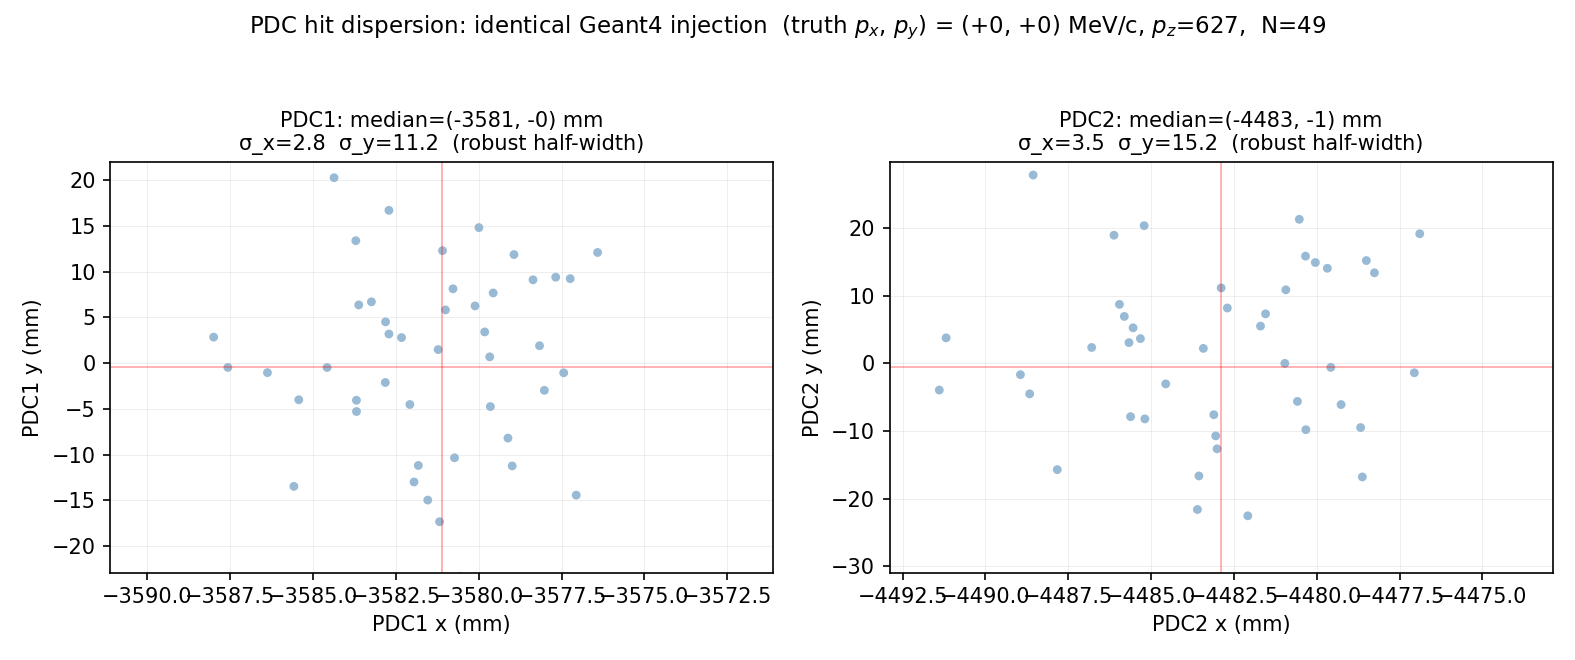
\includegraphics[width=0.96\textwidth]{figures/g4_fluctuation/pdc_hits/pxp0_pyp0.png}
\caption{$(p_x, p_y, p_z)=(0, 0, 627)$ MeV/$c$ 真值下 49 份 G4 重复事件的 PDC1/PDC2 命中散点。左 PDC1、右 PDC2。注意 $y$ 方向尺度仍是 $x$ 的 $\sim$4 倍；红线为 $p_{50}$ 中位数。关掉 Sn 靶后 $\sigma_y$ 从 $\sim$100 mm 降到 $\sim$10--15 mm。}
\label{fig:pdc_disp_0_0}
\end{figure}

\begin{figure}[H]
\centering
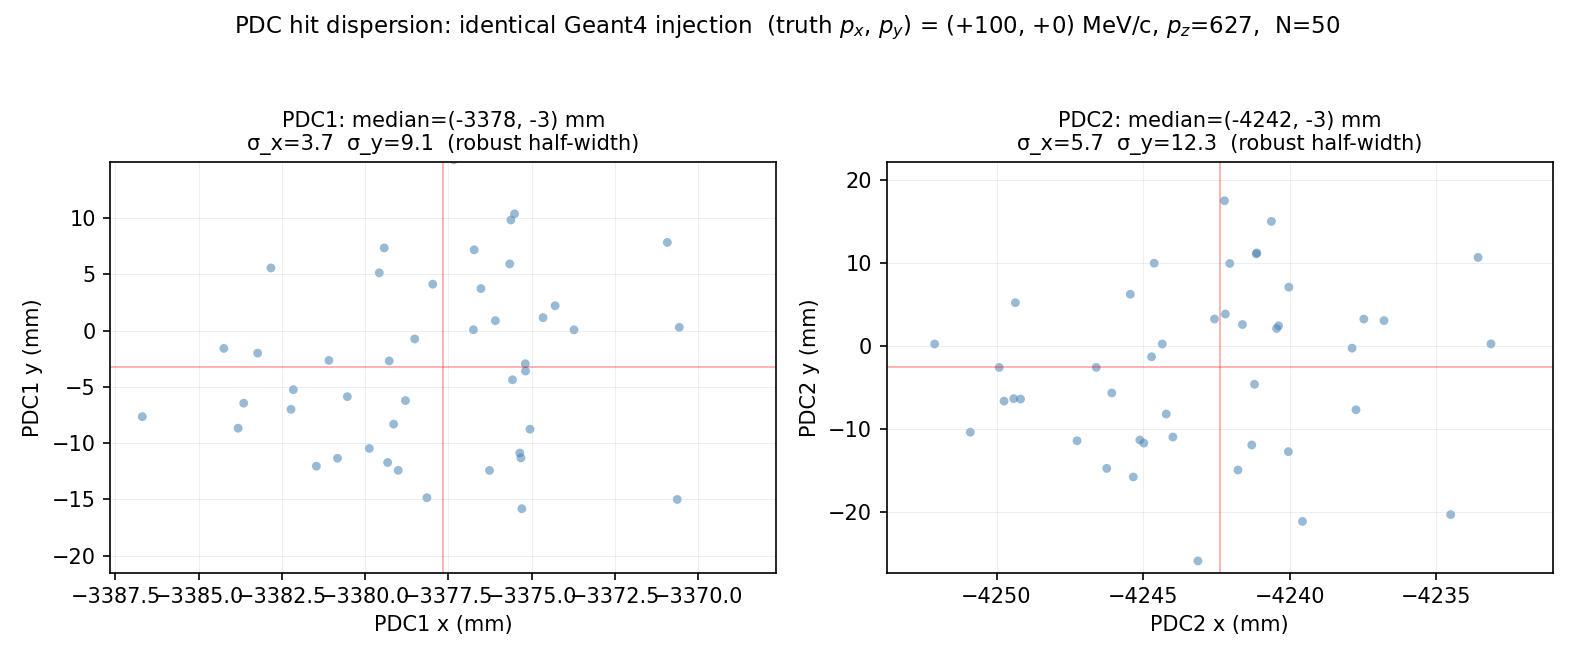
\includegraphics[width=0.96\textwidth]{figures/g4_fluctuation/pdc_hits/pxp100_pyp0.png}
\caption{$(+100, 0, 627)$ MeV/$c$ 真值下的同样对比。$\sigma_x$ 比 $(0,0)$ 略大（3.7/5.7 mm vs.\ 2.8/3.5 mm），$\sigma_y$ 略小（9.1/12.3 mm vs.\ 11.2/15.2 mm）。}
\label{fig:pdc_disp_100_0}
\end{figure}

\begin{figure}[H]
\centering
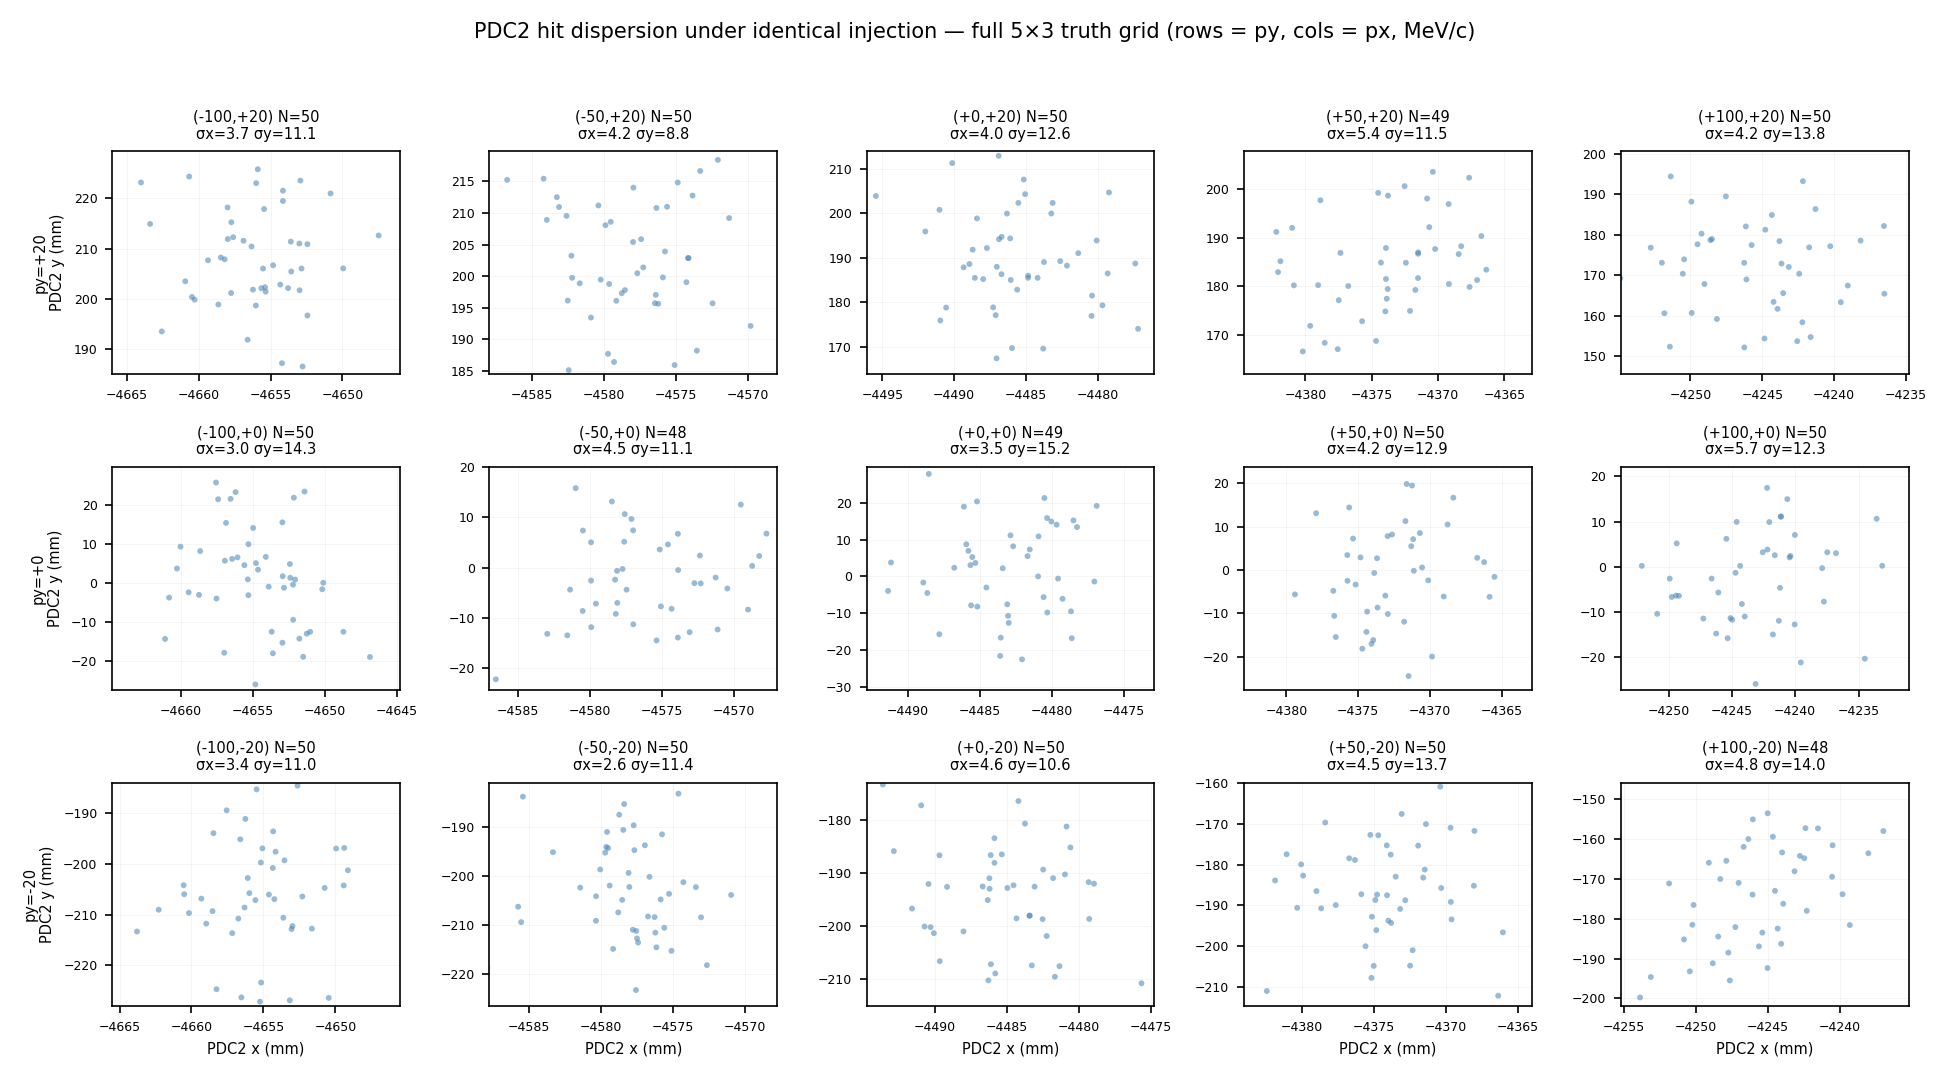
\includegraphics[width=0.99\textwidth]{figures/g4_fluctuation/pdc_hits/overview.png}
\caption{完整 $5\times 3$ 真值网格的 PDC2 命中弥散总览（行 $p_y \in \{+20, 0, -20\}$，列 $p_x \in \{-100,-50,0,50,100\}\;\mathrm{MeV}/c$）。每个格内是该真值点 $N{=}48$--$50$ 份 G4 重复事件的 PDC2 $(x,y)$ 散点，标注的是鲁棒半宽 $\sigma_x,\sigma_y$。PDC1 的数据见 \texttt{pdc\_dispersion\_summary.csv}。整个网格上 PDC 平面的 $\sigma_y$ 都在 $8$--$15$ mm 量级，$\sigma_x$ 在 $2$--$6$ mm——比 0.2 mm 的丝坐标涂抹大 $10$--$75\times$，但已经是关掉 Sn 靶之后"纯 PDC 气体 MS + 丝坐标噪声"的物理下限。\textbf{轨迹噪声仍主导测量噪声，但已是真实 PDC 追踪实验的 MS 水平。}}
\label{fig:pdc_disp_overview}
\end{figure}

% ============================================================
\subsubsection{第二步：PDC 命中弥散 $\to$ 重建动量弥散}
% ============================================================

\paragraph{传递关系。}
RK4 fitter 做的是 $\vec p_\mathrm{target} \mapsto (\vec r_\mathrm{PDC1}, \vec r_\mathrm{PDC2})$ 的逆向拟合。\textbf{Fisher 矩阵里假设的输入 $\sigma$ 只有 $\sigma_\mathrm{wire}\!\sim\!0.2$ mm}（丝坐标分辨率），据此算出的 Fisher $\sigma_p$ 是几 MeV/$c$。关掉 Sn 靶后 PDC 平面弥散降到 $3$--$15$ mm——仍比 $\sigma_\mathrm{wire}$ 大 $15$--$75\times$，但不再是带靶时 $\sim\!500\times$ 的灾难。

\paragraph{坐标系提示。}
以下所有 $p_x, p_y, p_z$ 直方图都在\textbf{靶系}下给出（见 \S\ref{sec:frame_convention}）。2026-04-19 修复前的图因缺少 lab$\to$target 的 $R_y$ 旋转而在 $p_x$ 上带有 $-p_z\sin\alpha \approx -627\times\sin 3^\circ \approx -33\;\mathrm{MeV}/c$ 的系统性偏差（pre-fix 版本 PNG 归档于 \texttt{ensemble\_n50\_with\_target\_backup/}），本节所有数字与 PNG 为修复后重跑版本（\texttt{ensemble\_n50\_targetframe/}）。

\paragraph{Fisher $\sigma$ 带和 Geant4 物理的边界。}
Fisher 矩阵的所有信息都来自 RK 前向模型：
\[
F \;=\; J^{\!\top}\,\Sigma_\mathrm{meas}^{-1}\,J,
\qquad
\Sigma_p^\mathrm{Fisher} \;=\; F^{-1},
\]
其中 $J = \partial\,(\vec r_\mathrm{PDC1},\vec r_\mathrm{PDC2})/\partial(p_x,p_y,p_z)$ 是最佳拟合点处的 RK Jacobian，$\Sigma_\mathrm{meas}$ 只装了 PDC 丝的位置协方差（$\sigma_\mathrm{wire}\!\sim\!0.2$ mm）。\textbf{Fisher 能看到的只有这两样}——测量噪声 + 确定性前向模型的一阶展开。

\vspace{0.05cm}
\textbf{Fisher 看不到的 Geant4 随机过程}（每一条都会把真实的重建散布推得比 Fisher $\sigma$ 更宽）：
\begin{itemize}\itemsep0pt
  \item PDC 气体、窗口、约 1 m 空气中的多次库仑散射（multiple scattering，MS）；
  \item 电离能损的 Landau/Vavilov 涨落——RK 传播只带 $dE/dx$ 的\emph{均值}；
  \item $\delta$ 电子产生、次级核反应；
  \item PDC 漂移气体 cluster 扩散的非高斯尾巴（$\sigma_\mathrm{wire}$ 是理想化的高斯）。
\end{itemize}

\vspace{0.05cm}
\textbf{ensemble 直方图才看得见完整物理}。固定真值 $(p_x,p_y,p_z)$、换 50 个随机种子独立跑 Geant4，直方图宽度就是 \emph{实测的} $\sigma_p^\mathrm{G4}$。这也是本节两张图（Step 1 PDC 弥散 + Step 2 reco 动量弥散）的存在意义：Fisher 给 \emph{预测}，G4 ensemble 给 \emph{真相}。

\vspace{0.05cm}
\textbf{G4/Fisher 比值 $r$ 的读法}：
\begin{itemize}\itemsep0pt
  \item $r \gg 1$ $\Rightarrow$ Geant4 物理（主要是 MS）在这个方向上贡献了 Fisher 看不见的散布。$p_y$ 在 $r\!\approx\!1.9$ 处就是这种情况——磁场在 $xz$ 平面里弯曲，$p_y$ 完全不受磁铁约束；PDC 气体里每一次 MS 踢都在 $y$ 上加一份 Fisher 无法预估的方差。
  \item $r \lesssim 1$ $\Rightarrow$ 假设的 $\sigma_\mathrm{wire}$ 比 G4 实际给出的 PDC 读数涨落偏保守。$p_x,\,p_z,\,|\vec p|$ 在 $r\!\approx\!0.8$ 就是这种情况：偶极约束足够强，丝测量噪声主导，而 $0.2$ mm 标称值略大于实际。
\end{itemize}

\vspace{0.05cm}
\textbf{结论}。想让 Fisher 看到 Geant4 物理，只能把过程协方差并入测量协方差：$\Sigma_\mathrm{meas} \to \Sigma_\mathrm{meas} + \Sigma_\mathrm{MS} + \Sigma_\mathrm{strag}$（Kalman/Gluckstern 径迹拟合的做法）。当前 RK 后端没有这一步，所以 $p_y$ Fisher $\sigma$ 系统性欠估 $\sim\!2\times$。Profile / MCMC 的输入和 Fisher 共用同一个前向模型，该欠估它们也逃不掉；真正的修法是 Cartesian 重参数 + 加入过程噪声。

\paragraph{逐点重建动量直方图。}
脚本：\texttt{scripts/analysis/plot\_reco\_momentum\_dispersion.py}。每点一张 1×3 子图（reco px / py / pz），黑竖线 = 真值、红虚线 = G4 中位数、粉带 = Fisher $\sigma$（围绕中位数）。

\begin{figure}[H]
\centering

\includegraphics[width=0.98\textwidth]{figures/g4_fluctuation/reco_momentum/pxp0_pyp0.png}
\caption{基线 $(0,0,627)$ 真值下 49 份 G4 重复事件的 reco $(p_x, p_y, p_z)$ 分布（靶系）。2026-04-19 修复后，$p_x$ 中位数已居中在 $+0.3\;\mathrm{MeV}/c$（修复前为 $-33\;\mathrm{MeV}/c$，就是漏了坐标系旋转），G4 $\sigma=4.5$ vs.\ Fisher $\sigma=7.1$，比值 0.63——Fisher 稍保守；$p_y$ G4=1.5 vs.\ Fisher=0.8，比值 1.96（这是真正的 Fisher 欠估方向）；$p_z$ 中位 $-1.3\;\mathrm{MeV}/c$、G4=4.4 vs.\ Fisher=6.3，比值 0.69。修复后 $p_x$ 已无系统偏差，余下只剩 $p_y$ Fisher 欠估和 $(u,v,p)$ 线性化残留。}
\label{fig:reco_disp_0_0}
\end{figure}

\begin{figure}[H]
\centering

\includegraphics[width=0.98\textwidth]{figures/g4_fluctuation/reco_momentum/pxp100_pyp0.png}
\caption{$(+100, 0, 627)$ 真值下 50 份 G4 重复事件（靶系）。修复后 $p_x$ 中位 $+0.03\;\mathrm{MeV}/c$（已居中），G4=3.8 vs.\ Fisher=6.7，比值 0.57（Fisher 稍保守）；$p_y$ G4=1.4 vs.\ Fisher=0.5，比值 2.78（15 个真值点中比值最大——Fisher $\sigma_{p_y}$ 最紧而 G4 典型）；$p_z$ G4=5.2 vs.\ Fisher=7.8，比值 0.67。不同真值点的 Fisher/残差比值确实有 $\sim 2\text{-}3\times$ 的点到点差异——下表汇总。}
\label{fig:reco_disp_100_0}
\end{figure}

\paragraph{全网格总览（5×3 真值点）。}
把所有 15 个真值点逐分量铺成 $3\times 5$ 矩阵，便于一眼比较 bias 与 $\sigma$ 随入射方向的变化。

\begin{figure}[H]
\centering
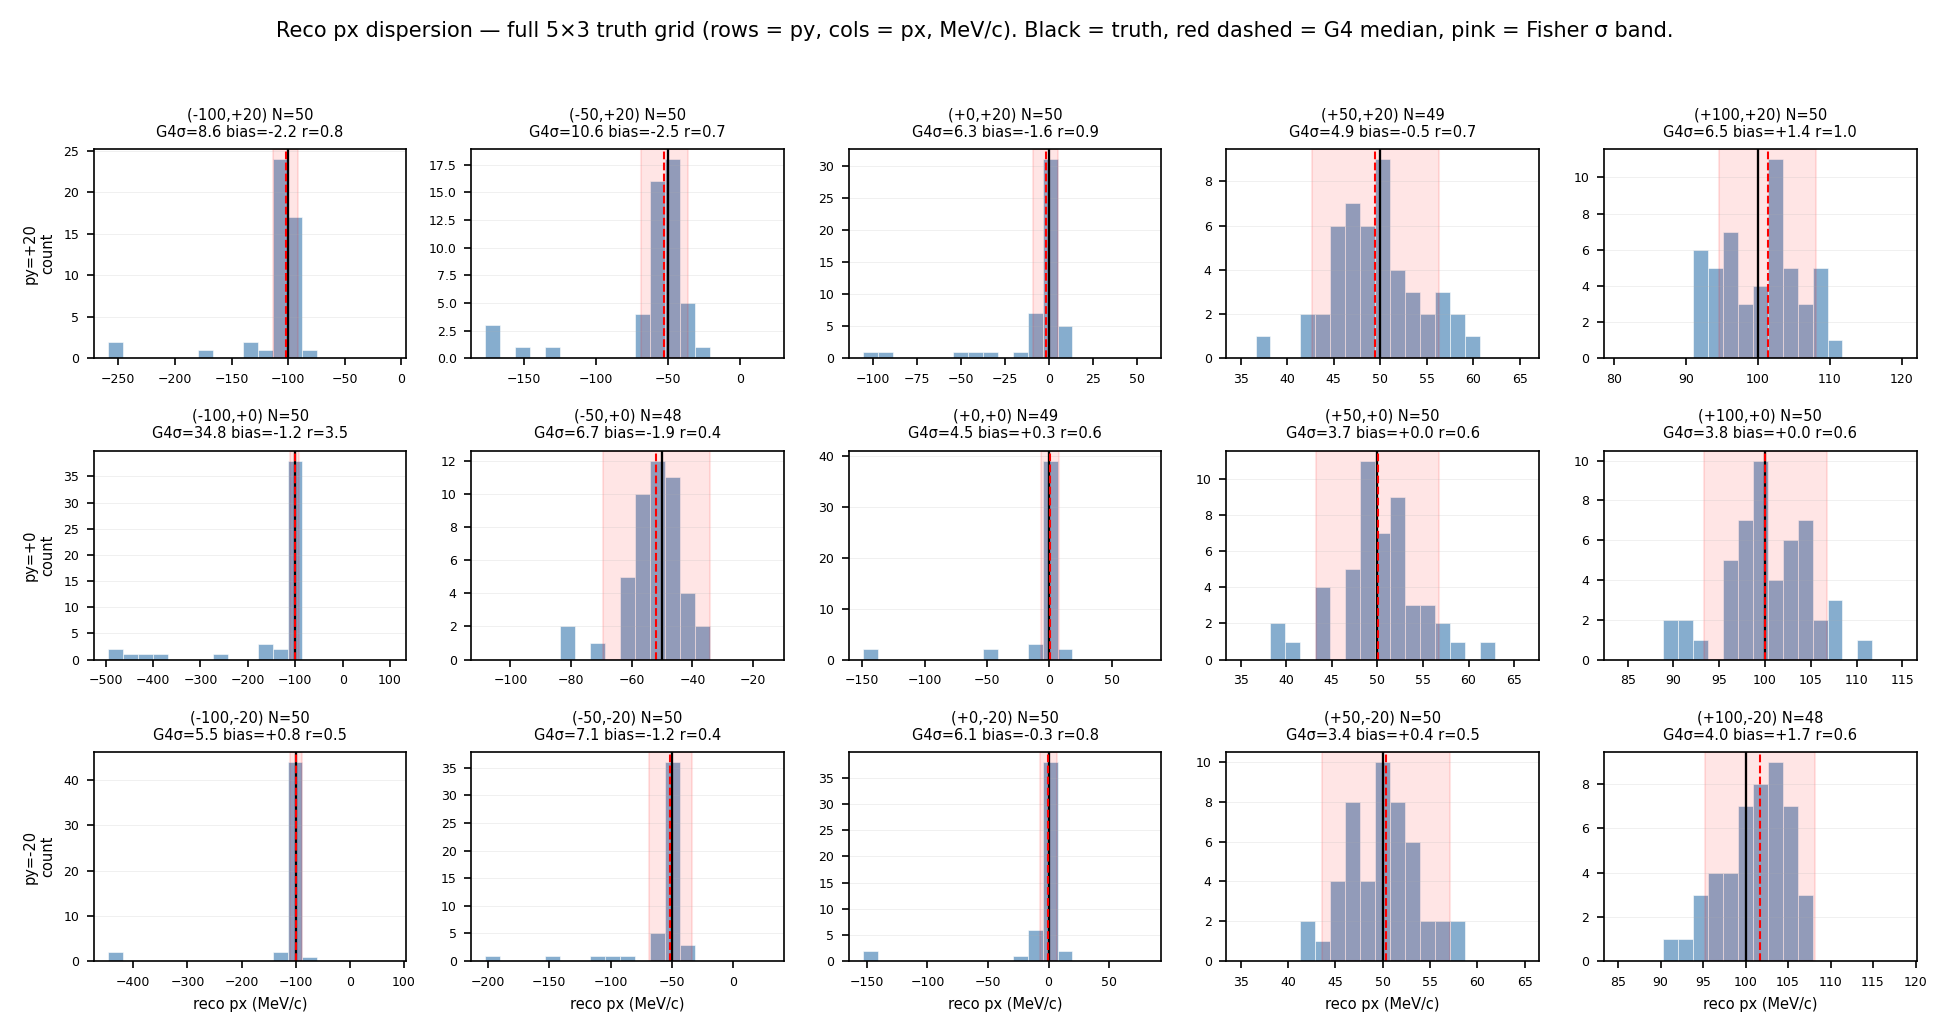
\includegraphics[width=0.99\textwidth]{figures/g4_fluctuation/reco_momentum/grid_px.png}
\caption{完整 $5\times 3$ 真值网格的 reco $p_x$ 直方图（靶系；行 $p_y \in \{+20,0,-20\}$，列 $p_x \in \{-100,-50,0,50,100\}\;\mathrm{MeV}/c$）。每格黑线 = 真值、红虚线 = G4 中位数、粉带 = Fisher $\sigma$；标注 $r$ = G4 $\sigma$ / Fisher $\sigma$。2026-04-19 修复后，中位偏差收敛到 $|\langle\Delta p_x\rangle| \lesssim 3\;\mathrm{MeV}/c$（修复前统一偏 $-30$ 到 $-40$，全盘是坐标系错误）；$(-100,0)$ 格仍是 LM 在 PDC 接收度边缘掉到粗格盆地的异常点，G4 $\sigma$ 飙到 $\sim 35\;\mathrm{MeV}/c$，比值 3.5。除该格外比值稳定在 $0.4$--$0.9$，\textbf{Fisher 大小基本正确、偏差已消除}，剩下主要是粗格 LM 盆地在极端动量点的散布。}
\label{fig:reco_disp_grid_px}
\end{figure}

\begin{figure}[H]
\centering
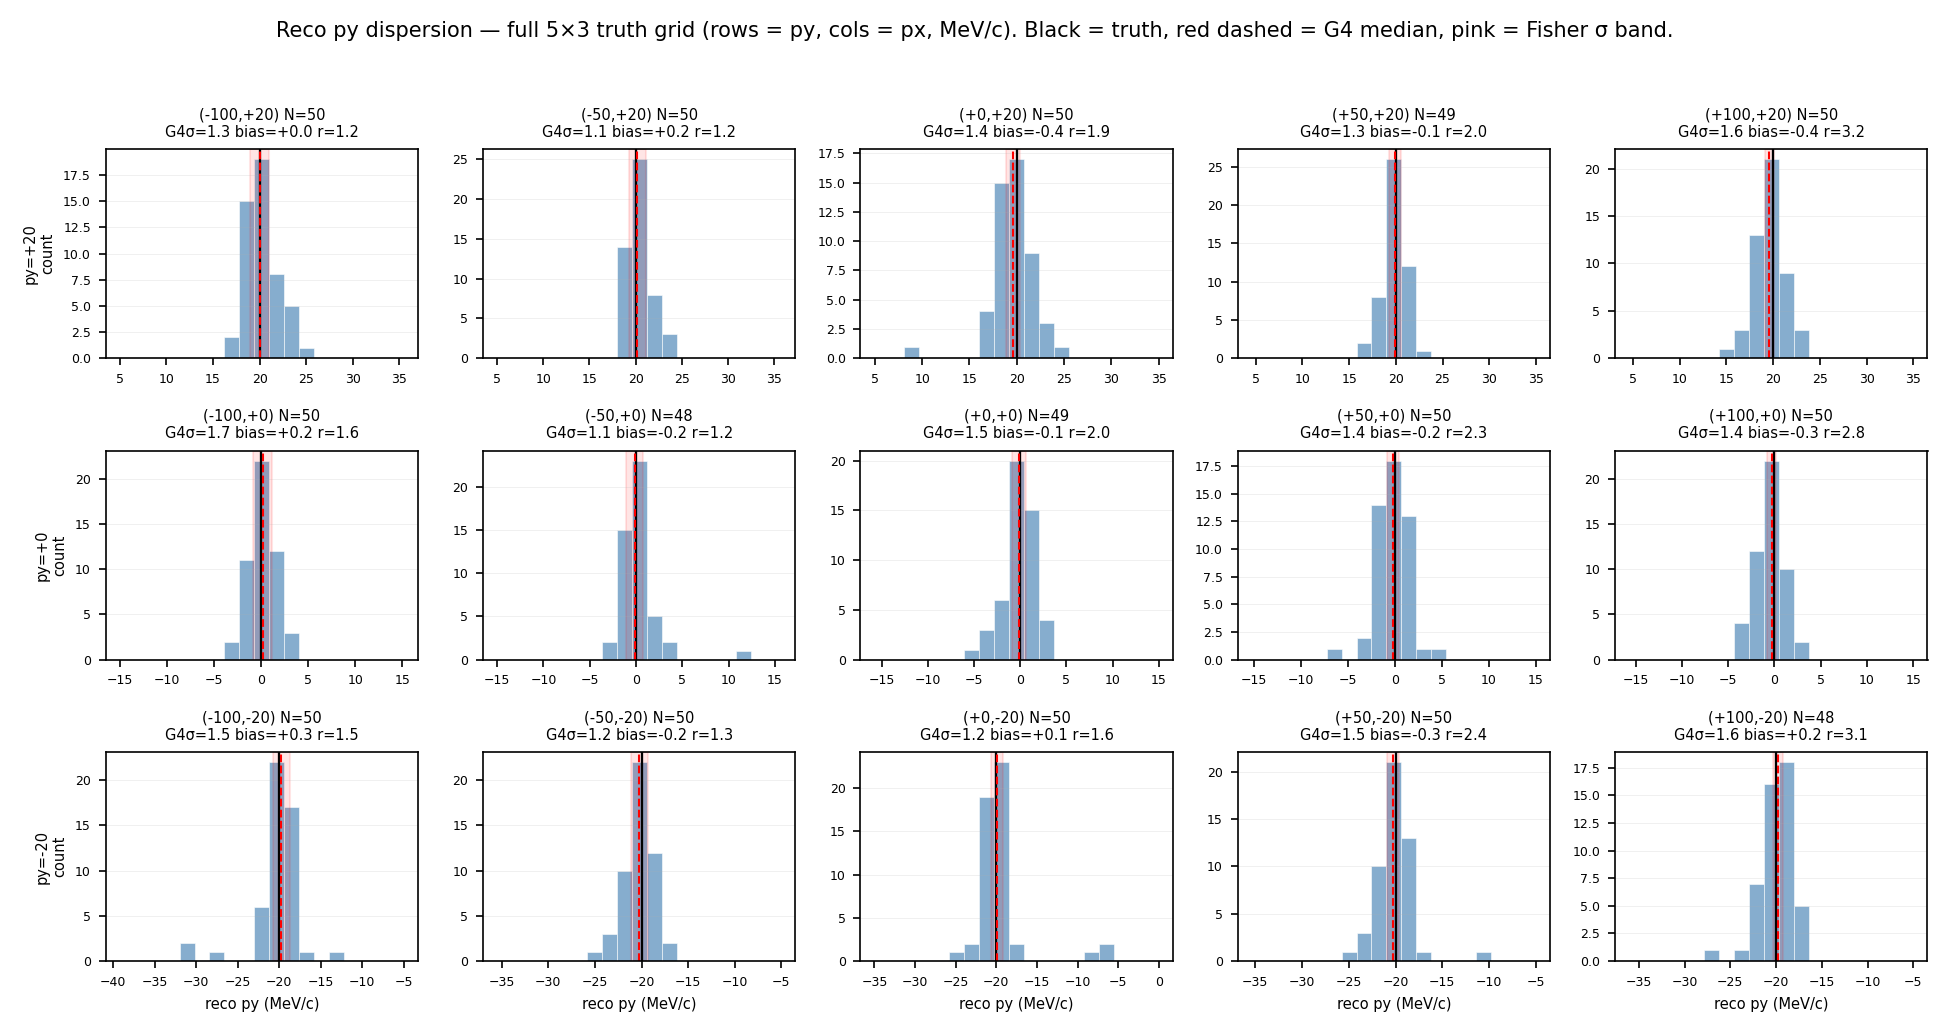
\includegraphics[width=0.99\textwidth]{figures/g4_fluctuation/reco_momentum/grid_py.png}
\caption{同样布局，分量改为 $p_y$（靶系）。$p_y$ 方向本就不受 $R_y$ 旋转影响，修复前后数字不变：G4 半宽 $1.1$--$1.7\;\mathrm{MeV}/c$，Fisher $\sigma_{p_y}$ 在 $0.5$--$1.0\;\mathrm{MeV}/c$，比值 $1.2$--$3.2$（全局中位 1.86）——这是 \textbf{Fisher $\sigma_{p_y}$ 系统性欠估 $\sim 2\times$} 的可视化证据。物理上归因于 $(u,v,p)$ 参数化把 $p_y$ 响应线性化后低估了实际传递涨落。中位偏差始终 $|\langle\Delta p_y\rangle| \lesssim 0.5\;\mathrm{MeV}/c$。}
\label{fig:reco_disp_grid_py}
\end{figure}

\begin{figure}[H]
\centering
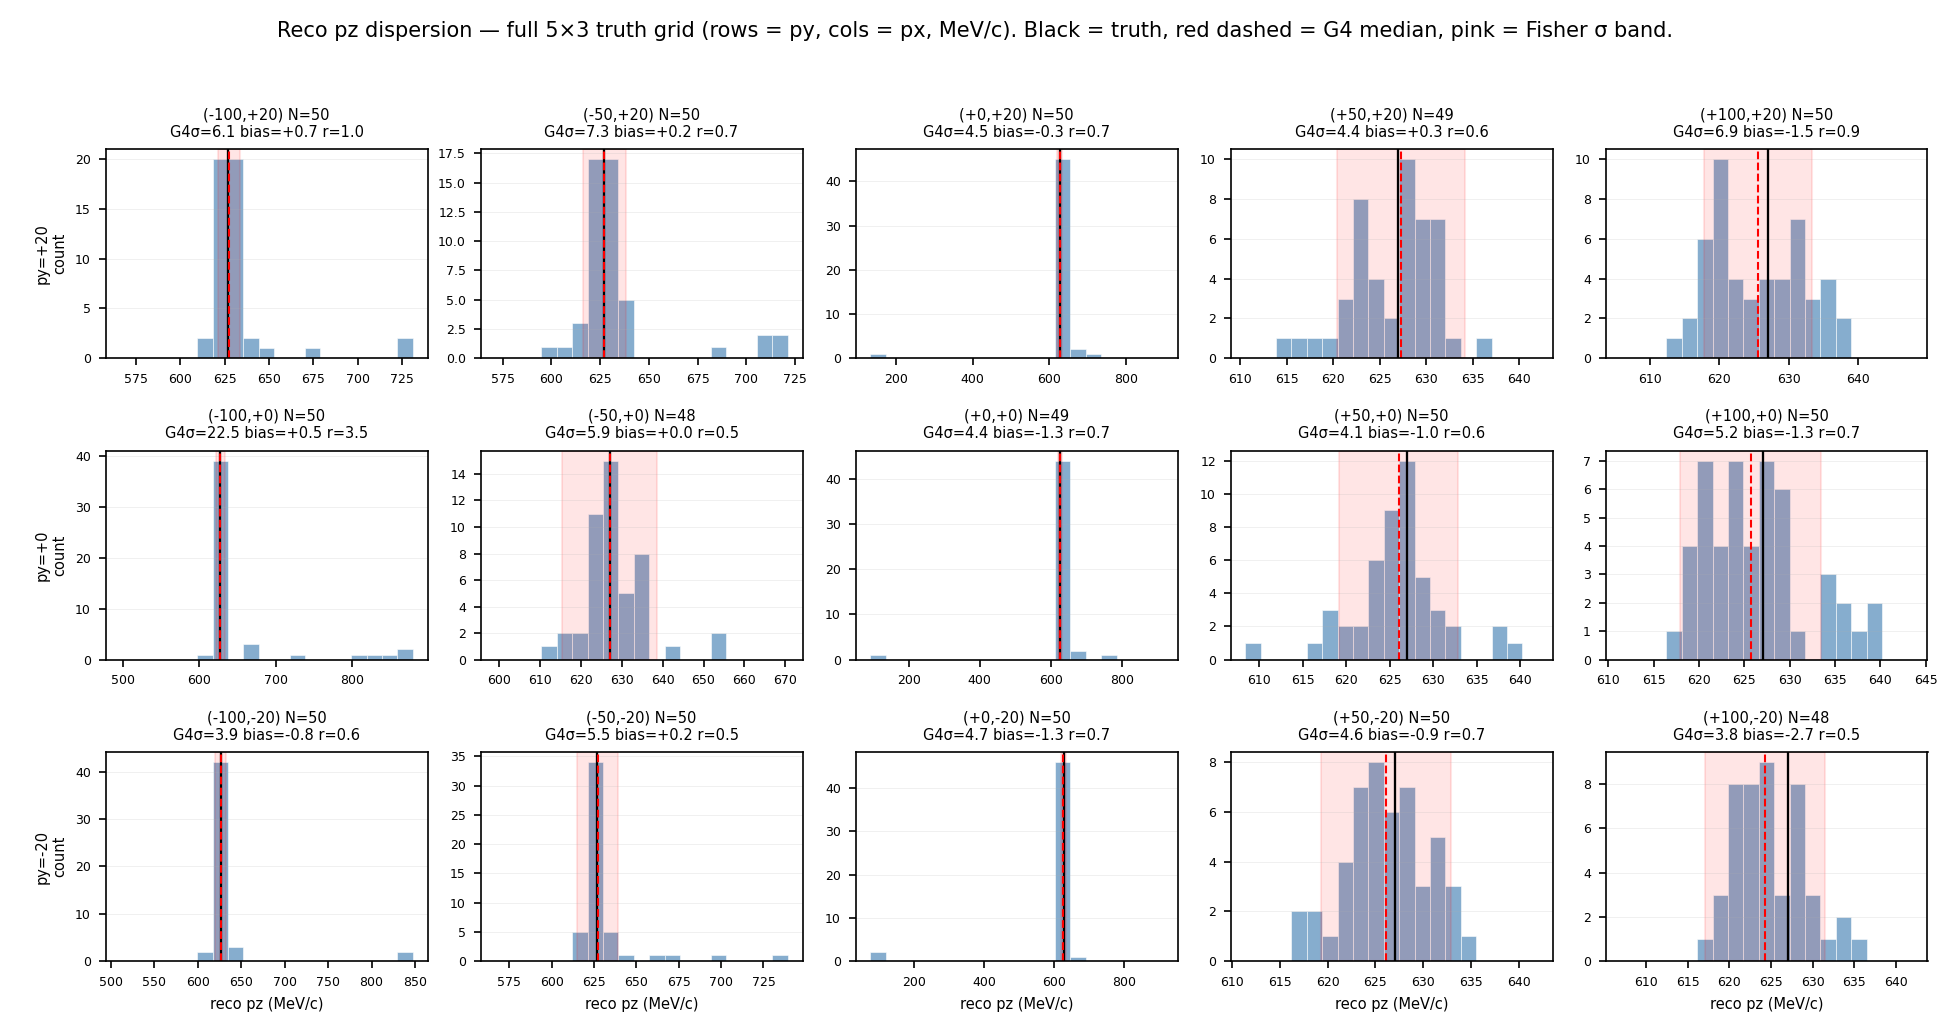
\includegraphics[width=0.99\textwidth]{figures/g4_fluctuation/reco_momentum/grid_pz.png}
\caption{同样布局，分量改为 $p_z$（靶系）。修复后整个网格 G4/Fisher 比值主要在 $0.5$--$0.9$（全局 0.80）——Fisher 对 $p_z$ \emph{略微保守}。中位偏差 $|\langle\Delta p_z\rangle| \lesssim 3\;\mathrm{MeV}/c$（修复前存在 $p_z\cos\alpha - p_z \approx -0.9\;\mathrm{MeV}/c$ 的小偏差，修复后消除）。唯一例外仍是 $(-100,0)$ 格：LM 拟合在 PDC 接收度边缘失败导致 G4 $\sigma\sim 22\;\mathrm{MeV}/c$，比值飙到 3.5。所有格的真值 $p_z=627\;\mathrm{MeV}/c$。}
\label{fig:reco_disp_grid_pz}
\end{figure}

\paragraph{PDC $\to$ 动量放大因子总表。}

\begin{table}[H]
\centering\footnotesize
\caption{PDC 平面弥散（第一步）与 reco 动量弥散（第二步）逐点对照（来源 \texttt{pdc\_dispersion\_summary.csv}、\texttt{reco\_momentum\_dispersion\_summary.csv}）}
\begin{tabular}{rr|rrrr|rrr}
\toprule
\multicolumn{2}{c}{真值} & \multicolumn{4}{c}{PDC 弥散 (mm)} & \multicolumn{3}{c}{G4 / Fisher 比值} \\
\cmidrule(lr){3-6}\cmidrule(lr){7-9}
$p_x$ & $p_y$ & $\sigma^{1}_x$ & $\sigma^{1}_y$ & $\sigma^{2}_x$ & $\sigma^{2}_y$ & $p_x$ & $p_y$ & $p_z$ \\
\midrule
$0$    & $0$   & 2.8 & 11.2 & 3.5 & 15.2 & 0.63 & 1.96 & 0.69 \\
$+100$ & $0$   & 3.7 &  9.1 & 5.7 & 12.3 & 0.57 & 2.78 & 0.67 \\
$-100$ & $0$   & 2.7 & 10.7 & 3.0 & 14.3 & 3.51 & 1.63 & 3.51 \\
$0$    & $+20$ & 2.9 &  9.6 & 4.0 & 12.6 & 0.89 & 1.90 & 0.72 \\
$0$    & $-20$ & 3.2 &  8.4 & 4.6 & 10.6 & 0.84 & 1.61 & 0.73 \\
\bottomrule
\end{tabular}
\end{table}

\paragraph{横向读表。}
\begin{itemize}[nosep]
  \item 关掉 Sn 靶后 PDC $\sigma_y$ 从 $\sim$100 mm 塌到 $\sim$10--15 mm，对应 reco 动量 G4/Fisher 比值也从老版本的 $3$--$28\times$ 塌到 $p_x,p_z$ 的 $\sim 0.6$--$0.9$ 和 $p_y$ 的 $\sim 1.5$--$3$——\emph{Fisher 宽度定标基本正确}，唯一剩余的宽度问题在 $p_y$。
  \item $(-100, 0)$ 是单独失控的一个点：$p_x / p_z$ G4 半宽分别飙到 $\sim 35$ 和 $\sim 22\;\mathrm{MeV}/c$（比值 $3.5$）——这就是 LM 粗格 + PDC 接收度边缘"向内偏转"轨迹的已知覆盖率盲区（见项目 memo 中 RK 覆盖率报告）。
  \item 2026-04-19 坐标系修复后，原先 $p_x$ 中位偏差 $\sim\!-33\;\mathrm{MeV}/c$ 的系统性拉偏已消除（现在 $|\langle\Delta p_x\rangle| \lesssim 3\;\mathrm{MeV}/c$），修复前归咎给"前向模型居中位置"的 $p_x$ 欠覆盖部分其实是 lab/靶系混用。修复后 Fisher 68\% 覆盖率 $p_x$ 0.80 / $p_z$ 0.77 / $|\vec p|$ 0.76 均在名义 0.68 附近，Profile/MCMC 结果一致。剩余 $p_y$ Fisher $\sigma$ 压低 $\sim 1.9\times$ 来自 $(u,v,p)$ 线性化——仍需要 $dE/dx$ + Cartesian $(p_x,p_y,p_z)$ 直接拟合来根治。
\end{itemize}

% ============================================================
\section{代码架构与关键文件}
% ============================================================

\begin{table}[H]
\centering
\caption{关键源文件一览}
\small
\begin{tabular}{p{7cm}p{7cm}}
\toprule
文件路径 & 功能 \\
\midrule
\texttt{libs/analysis\_pdc\_reco/src/}\ & \\
\quad\texttt{PDCRkAnalysisInternal.cc/hh} & RK 最小二乘分析器：参数化、残差构建、白化、LM 迭代、网格搜索、多起点、Fisher/Laplace \\
\quad\texttt{PDCMomentumReconstructorRK.cc} & 三种 RK 模式的入口（统一委托给 Analyzer） \\
\quad\texttt{PDCErrorAnalysis.cc/hh} & 误差分析：MC 传播、Profile Likelihood、MCMC、丝坐标扰动 \\
\midrule
\texttt{libs/analysis/src/}\ & \\
\quad\texttt{ParticleTrajectory.cc} & RK4 积分器、洛伦兹力计算 \\
\quad\texttt{PDCSimAna.cc} & PDC 丝坐标定义与重建 \\
\midrule
\texttt{apps/run\_reconstruction/main.cc} & 重建 CLI 入口 \\
\texttt{apps/tools/analyze\_pdc\_rk\_error.cc} & 离线误差分析 CLI \\
\texttt{tests/analysis/test\_PDCMomentum\dots.cc} & 单元测试（6 项） \\
\texttt{tests/analysis/test\_PDCErrorAnalysis.cc} & 误差分析测试（4 项） \\
\bottomrule
\end{tabular}
\end{table}

% ============================================================
\section{已知局限与后续工作}
% ============================================================

\begin{enumerate}
  \item \textbf{$dE/dx$ 能量损失}（优先级高）。在 RK4 步进中添加 Bethe-Bloch 连续能量损失项。预期可消除 $p_z$ 的 $5\text{--}16\;\mathrm{MeV}/c$ 系统负偏差。改动位置：\texttt{ParticleTrajectory::RungeKuttaStep()}。

  \item \textbf{多重散射}。探测器气体和窗口材料中的库仑散射引入角度弥散（$\sim\!\mathrm{mrad}$ 量级），可作为轨迹模型的过程噪声引入。对 $635\;\mathrm{MeV}/c$ 质子影响有限，但精密测量时不可忽略。

  \item \textbf{修复欠覆盖}（2026-04-19 坐标系修复后更新）。744 事件（关掉 Sn 靶、修复 lab$\to$target 旋转后）ensemble 显示 Fisher 68\% 覆盖率 $p_x\,80\%$、$|\vec p|\,76\%$、$p_z\,77\%$（$p_x$ 从修复前 $5\%$ 直接恢复——原因是坐标系而非前向模型），$p_y\,42\%$（Fisher 偏紧 $1.9\times$，这是真正剩下的算法级短板；$p_y$ 不受 $R_y$ 影响，修复前后数字一致）。在扩大数据集之前仍需：
  \begin{itemize}[nosep]
    \item 把 $(u,v,p)$ 参数化改为 Cartesian $(p_x,p_y,p_z)$ 直接拟合（当前版本未实现，见已知局限 \#5）——目标是把 $p_y$ Fisher $\sigma$ 从 $0.75$ 提到 $\sim 1.4\;\mathrm{MeV}/c$；
    \item 在修复后的 \texttt{profile\_samples.csv}/\texttt{bayesian\_samples.csv} 上重算 Profile/MCMC 覆盖率（预期 $p_x$ Profile 从 $0\%$ 恢复到 $\gtrsim 70\%$）；
    \item 消除 $p_z$ 系统偏差（见上条 $dE/dx$）。
  \end{itemize}
  修复后再在 $89\mathrm{k}$ 事件 NN 训练集上做大统计验证，目标 $p_x,p_z$ 稳定在 $[65\%, 75\%]$，$p_y$ 需要 Cartesian 改造后才能达标。

  \item \textbf{E2E 测试门限}。当大统计验证通过后，将 \texttt{require\_gate\_pass} 从 0 改为 1，启用硬门禁。

  \item \textbf{$(p_x, p_y, p_z)$ 并行参数化拟合器}（已立项，未实现）。\texttt{RecoConfig::rk\_parameterization} 已加入枚举开关（\texttt{kDirectionCosines} 默认 / \texttt{kCartesian}），Cartesian 版 LM 分析器尚未写。当前覆盖率结果基于 $(u,v,p)$ 参数化；并行 Cartesian 路径作为诊断能暴露参数化诱导的系统误差。详见 \texttt{docs/reports/reconstruction/rk\_reconstruction\_bugfix\_and\_error\_analysis\_20260416.md} 的 Phase 1 计划。

  \item \textbf{自适应 RK 步长}。当前使用固定 $\Delta t$，可引入 RK45（Dormand-Prince）自适应步长控制，在磁场梯度剧烈区域自动缩小步长。
\end{enumerate}

% ============================================================
\section{结论}
% ============================================================

本报告详细描述了 PDC 靶点动量重建管线的当前状态：

\begin{enumerate}
  \item \textbf{物理过程}：质子从靶点出发，在 SAMURAI 偶极磁场（$1.15\;\mathrm{T}$，旋转 $30^\circ$）中偏转约 $25^\circ$，依次穿过 PDC1（$z \approx 4000\;\mathrm{mm}$）和 PDC2（$z \approx 5000\;\mathrm{mm}$）。两组漂移室提供 $u$、$v$ 丝坐标，编码了轨迹曲率与动量信息。

  \item \textbf{重建算法}：以 $(u, v, p)$ 或 $(\delta x, \delta y, u, v, p)$ 为参数，RK4 轨迹传播 + 丝坐标残差白化 + Levenberg-Marquardt 优化。粗网格搜索（105 候选）+ 多起点（5 个）策略解决了磁场偏转导致的初始化困难。

  \item \textbf{误差分析}：六种方法覆盖从快速近似（Fisher，$< 5\;\mathrm{ms}$/事件）到完整后验（MCMC，$\sim 5.5\;\mathrm{s}$/事件），包括非线性传播（MC 256 采样）和频率学置信区间（Profile Likelihood）。

  \item \textbf{当前精度}（来自 E2E 测试 CSV）：RK MAE = $(20.4,\;16.0,\;10.8)\;\mathrm{MeV}/c$（$p_x, p_y, p_z$），NN MAE = $(21.0,\;15.6,\;3.1)\;\mathrm{MeV}/c$。Fisher $\sigma_{|\vec{p}|}$ = 2.4--6.0 MeV/$c$。$p_z$ 残余系统偏差（均值 $-10.8\;\mathrm{MeV}/c$）源于未建模的 $dE/dx$ 能量损失。

  \item \textbf{理论极限}：出射角法 $\sigma_p \approx 1.0\text{--}4.1\;\mathrm{MeV}/c$（纯几何），加入多重散射后 $\sigma_p \approx 3.2\text{--}5.1\;\mathrm{MeV}/c$（Highland 公式计算，见第~\ref{sec:theory}~节）。NN 的 $p_z$ MAE = 3.1 MeV/$c$ 已接近理论极限。
\end{enumerate}

\end{document}
